\documentclass[12pt,openany]{report}
\usepackage[UTF8,fontset=fandol]{ctex}
\usepackage{amsmath}
\usepackage[table]{xcolor}
\usepackage{graphicx}
\usepackage{subcaption}
\usepackage{booktabs}
\usepackage{float}
\usepackage{multirow}
\usepackage[hidelinks]{hyperref}
\usepackage{pdfpages}
\usepackage{enumitem}
\usepackage{setspace}
\usepackage{fancyhdr}
\usepackage{titlesec}
\usepackage[a4paper,left=2.6cm,right=2.6cm,top=2.8cm,bottom=2.8cm]{geometry}
\usepackage[super,sort&compress]{natbib}

\graphicspath{{images/}}
\onehalfspacing
\AtBeginDocument{\zihao{-4}}
\setlength{\parindent}{2em}
\setlength{\parskip}{0pt}
\setlength{\headheight}{15pt}
\captionsetup{font={small},labelfont=bf,textfont=normalfont,labelsep=space,justification=centering}
\titleformat{\chapter}[block]{\centering\bfseries\zihao{3}}{第\,\thechapter\,章}{1em}{}
\titlespacing*{\chapter}{0pt}{0.5\baselineskip}{0.5\baselineskip}
\titleformat{\section}[block]{\bfseries\zihao{4}}{\thesection}{0.75em}{}
\titlespacing*{\section}{0pt}{0.5\baselineskip}{0.5\baselineskip}
\titleformat{\subsection}[block]{\bfseries\zihao{-4}}{\thesubsection}{0.75em}{}
\titlespacing*{\subsection}{0pt}{0.5\baselineskip}{0.5\baselineskip}
\titleformat{\subsubsection}[runin]{\bfseries\zihao{-4}}{\thesubsubsection}{0.75em}{}[。]
\pagestyle{fancy}
\fancyhf{}
\fancyhead[C]{{\zihao{-5} 南京师范大学计算机与电子信息学院本科毕业论文}}
\renewcommand{\headrulewidth}{0.4pt}
\fancyfoot[C]{\zihao{-5}\thepage}
\fancypagestyle{plain}{
  \fancyhf{}
  \fancyhead[C]{{\zihao{-5} 南京师范大学计算机与电子信息学院本科毕业论文}}
  \renewcommand{\headrulewidth}{0.4pt}
  \fancyfoot[C]{\zihao{-5}\thepage}
}
\renewcommand{\bibsection}{\section*{参考文献}\addcontentsline{toc}{section}{参考文献}}

\newcommand{\best}[1]{\textcolor{green!45!black}{\textbf{#1}}}
\newcommand{\worst}[1]{\textcolor{red!75!black}{\textbf{#1}}}
\newcommand{\secondbest}[1]{\textcolor{green!45!black}{#1}}
\newcommand{\secondworst}[1]{\textcolor{red!75!black}{#1}}
\newcommand{\focusval}[1]{\textbf{#1}}
\newcommand{\upperbase}[1]{\textcolor{green!45!black}{\textbf{#1}}}
\newcommand{\lowerbase}[1]{\textcolor{red!75!black}{\textbf{#1}}}
\newcommand{\modelcap}[1]{\textcolor{blue!70!black}{\textbf{#1}}}
\newcommand{\thesistitle}{基于混合检索器的多模态生成模型研究与实现}
\newcommand{\thesisauthor}{时子延}
\newcommand{\thesisid}{19220422}
\newcommand{\thesismajor}{人工智能}
\newcommand{\thesiscollege}{计算机与电子信息学院/人工智能学院}
\newcommand{\thesisadvisor}{宋歌}

\begin{document}
\setcounter{tocdepth}{2}


\includepdf[pages=-,fitpaper=true,pagecommand={\thispagestyle{empty}}]{时子延毕业论文封面.pdf}
\clearpage

\pagestyle{plain}
\pagenumbering{Roman}

\begin{center}
{\zihao{3}\bfseries 摘\quad 要\par}
\end{center}
\addcontentsline{toc}{chapter}{摘\texorpdfstring{\quad}{ }要}
\noindent\hspace*{\parindent}%
在以视觉为中心的多模态检索增强生成（vision-centric mRAG）任务中，下游多模态模型能否正确作答，往往首先受限于外部视觉证据是否被准确召回。与文本 RAG 主要补充事实知识不同，本文关注的任务要求系统根据查询图像与问题文本，从外部图像库中找到能够补足回答所需信息的候选证据图像；因此，检索目标不再是一般意义上的视觉相似图像，而是对当前问题有帮助的图像证据。围绕这一检索瓶颈，本文以 MRAG-Bench 为核心平台，对其候选字段、视觉证据覆盖和场景分布进行再统计，发现数据集给定候选与人工标注正例证据并不等价：44.12\% 的样本二者完全无重叠，平均 GT 覆盖率仅为 22.78\%。这一结果说明，若不区分局部重排与真实全库检索，容易混淆候选覆盖能力和候选排序能力。

基于上述分析，本文将实验设计为局部重排、全库检索与查询侧扩展三个部分，并将 E8 作为本文主要系统架构：利用 Gemma~4 根据查询图像、题干与选项生成五条互补检索维度，驱动 MagicLens 在完整图像库上分路召回，再通过 RRF 列表融合得到最终证据集合，并交由 LLaVA-OneVision 完成多选题终答。所有实验均固定下游 VLM 与提示模板，使性能差异主要归因于检索与查询构造环节。全量 MRAG-Bench 测试集结果表明，E8 在 1353 个样本上达到 56.32\% 准确率，是本文非 GT 全库检索路线中的最佳结果；相较 MagicLens direct retrieval（E7）提升 8.35 个百分点，相较 CLIP corpus RAG（E3）提升 5.91 个百分点。与此同时，人工标注证据路线 E1/E5 仍保持约 60.16\% 的参考上界，说明查询侧扩展显著改善了真实全库检索效果。

除最终准确率外，本文还引入前五候选重叠数（Top-5 overlap，指两种检索设置的前五候选中相同图像的数量）、首位一致率（Top-1 match，指两种设置的第一名候选是否一致）、逐样本胜负统计、高频重复命中分布与 E8/E9 样本级过程记录等分析指标。实验观察到，CLIP 与 MagicLens 在 67.2\% 的样本上 Top-5 候选完全不重合，说明二者具有显著不同的检索偏好；MagicLens 还存在 Top-1“原型图吸附”偏置，部分高响应图像被大量不同查询重复命中。E8 的过程记录进一步显示，五维检索产生的 25 个候选在 RRF 融合前平均保留 19.35 个唯一候选，94.75\% 的样本存在跨维重复命中，说明多维查询确实形成了可融合的证据共识。E9 在保持同一检索侧框架、仅将终答器替换为 Gemma~4~E2B-it 后降至 38.95\%，说明最终 VLM 的多图证据整合能力同样是系统瓶颈。本文建立了包含 benchmark 复现、候选覆盖再分析、E0--E9 实验线组织、样本级过程记录、可视化图表和错误模式分析在内的统一评测方法。

{\small\noindent\textbf{关键词：}多模态检索增强生成；混合检索；MRAG-Bench；MagicLens；查询链编排\par}

\clearpage
\begin{center}
{\zihao{3}\bfseries Abstract\par}
\end{center}
\addcontentsline{toc}{chapter}{Abstract}
\noindent\hspace*{\parindent}In vision-centric multimodal retrieval-augmented generation (mRAG), final answer quality is often bounded by whether the system can retrieve useful external visual evidence. Unlike text RAG, this task requires retrieving evidence images that help answer a question conditioned on both the query image and the question text. This thesis uses MRAG-Bench as the evaluation platform and re-analyzes its candidate fields, evidence coverage, and scenario distribution. The analysis shows that provided retrieved candidates and human-annotated ground-truth evidence are not equivalent: 44.12\% of samples have no overlap, and the average GT coverage is only 22.78\%. This motivates a clear separation between local reranking and full-corpus retrieval.

The experiments are organized into a reranking line, a corpus retrieval line, and a query-side extension line. The E8 pipeline is the main architecture: Gemma~4 generates five complementary retrieval dimensions from the query image, question, and choices; MagicLens performs per-dimension full-corpus retrieval; reciprocal rank fusion (RRF) produces the final evidence set; and a fixed LLaVA-OneVision model predicts the answer. On the full MRAG-Bench test split of 1,353 samples, E8 reaches 56.32\% accuracy, the best non-GT full-corpus retrieval result in this work. It improves over MagicLens direct retrieval (E7) by 8.35 percentage points and over CLIP corpus RAG (E3) by 5.91 points, while settings using human-annotated evidence in E1/E5 still reach 60.16\%.

Beyond accuracy, this thesis introduces Top-5 overlap, Top-1 match rate, per-sample win/loss statistics, repeated Top-1 hit analysis, and sample-level process records for E8/E9. CLIP and MagicLens return disjoint Top-5 candidates on 67.2\% of samples, showing different retrieval preferences. MagicLens also exhibits a Top-1 prototype-attraction bias, where a small number of high-response images are repeatedly retrieved. E8 records show that five-dimensional retrieval keeps 19.35 unique candidates on average before fusion and that 94.75\% of samples contain cross-dimension repeated hits. E9 keeps the same retrieval side but replaces the answerer with Gemma~4~E2B-it, dropping to 38.95\%, which shows that multi-image evidence integration by the final VLM is also a bottleneck. Overall, this work provides a reproducible evaluation framework covering benchmark reproduction, E0--E9 experiments, sample-level records, visualization, and error-mode analysis.

{\small\noindent\textbf{Key words:} multimodal RAG; hybrid retrieval; MRAG-Bench; MagicLens; query planning\par}

\tableofcontents
\clearpage
\pagestyle{fancy}
\pagenumbering{arabic}

\chapter{绪论}

\section{研究背景及研究意义}

\subsection{多模态检索增强生成任务背景}

以 Transformer 为基础的大规模语言模型（LLM）推动了自然语言理解、推理和生成任务的发展\cite{vaswani2017attention,minaee2024llm}。这类模型通过大规模预训练和指令微调获得了丰富的参数化知识，但其知识边界仍受训练语料、时间截断和模型参数容量限制。在面向专业领域、实时事件或长尾对象的应用中，仅依赖模型内部记忆往往难以保证回答的可验证性。

检索增强生成（Retrieval-Augmented Generation, RAG）通过在生成前显式访问外部知识库，将用户输入与检索证据共同交给生成模型，从而缓解参数化知识的时效性缺陷与证据不可追溯问题\cite{lewis2020rag,gao2023rag}。这一范式把模型回答从完全依赖内部参数，转向依赖可检索、可更新、可审计的外部证据。对于开放域问答、专业文档问答和事实核查任务，RAG 的关键问题在于回答依据是否能够被外部证据支撑、追溯和更新。

多模态大模型的发展使外部证据从文本扩展到图像、表格、文档和视频等模态，多模态检索增强生成（Multimodal RAG, mRAG）由此成为重要研究方向\cite{mei2025multimodalrag,abootorabi2025ask}。在多模态任务中，证据对象不再只是“相关文本段落”，而可能是某个角度的图像、某一时间状态的视觉记录，或能够补足结构信息的外部图片。检索器需要判断的也不只是语义相关性，而是证据是否能够支撑下游模型完成当前问题。

本文关注的视觉中心型多模态检索增强生成更进一步：很多问题不是让模型直接看一张图回答，而是要求系统先从外部图像库中找回辅助证据，再由下游视觉语言模型给出答案。此时，外部视觉证据是否被正确召回，会比生成模型本身的语言能力更直接地限制回答可靠性。换言之，vision-centric mRAG 的核心瓶颈并非单纯“模型是否会生成”，而是“系统是否找到了值得生成模型参考的候选证据图像”。

\subsection{现有问题的分析}

多模态大模型虽然能够同时处理图像与文本输入，但知识冻结和幻觉问题并未消失。知识冻结指模型训练语料存在时间边界，面对新知识、领域私有知识和长尾对象时容易给出过时或不可验证的回答\cite{gao2023rag}。幻觉则指模型在证据不足或证据冲突时生成表面合理但事实错误的内容。在多模态问答中，幻觉不仅表现为文本事实错误，还会具体表现为对象错配、属性错配、关系错配、时间状态错配、视角错配以及结构信息缺失导致的误判\cite{li2023pope}。

这些错误形式说明，多模态问答中的证据需求往往具有明确的视觉条件。例如，视角变化和局部可见性会影响对象识别，时间状态变化会影响同一对象在不同时刻的判断，结构缺失则要求系统寻找能够补全缺口的外部图像。若检索器返回的候选证据图像本身偏离任务需求，下游视觉语言模型即使具备较强的单图理解能力，也可能被噪声证据引导到错误答案。因此，在 mRAG 系统中，检索质量不是生成前的辅助环节，而是决定证据边界和回答可靠性的关键因素。

RAG 与 mRAG 的系统形态已经从简单的“检索后拼接上下文”，发展为同时涉及检索规划、模态选择、跨模态对齐、证据排序和生成控制的复杂流程\cite{mei2025multimodalrag,abootorabi2025ask}。与此同时，智能体（Agent，指可自主调用工具并执行多步任务的系统组件）、模型上下文协议（MCP，Model Context Protocol，用于统一模型与外部工具/数据源交互的协议）和技能模块（Skills，指可复用的任务能力封装）等工程机制也推动了外部工具和外部知识协同使用的系统落地\cite{wang2023agent,anthropic2024mcp,anthropic2024claudecode,langchain2024skills}。这些发展说明，检索器已经不只是模型前端的相似度搜索模块，而是连接任务意图、外部证据和最终生成的重要接口。

在图像证据参与的任务中，传统最近邻检索不能完全满足需求。本文真正要处理的不是通用图像检索（generic image retrieval），而是问题条件证据检索（question-conditioned evidence retrieval）。在这类任务中，查询图像既不是最终证据，也不是唯一检索条件；问题文本决定了系统究竟需要补足哪一种视觉信息，因此检索目标（retrieval target）从视觉相似图像（visually similar image）转变为对答案有用的证据图像（answer-useful evidence image）。这一转变要求研究者同时关注视觉语义近邻、图像间关系、问题文本约束和候选证据可用性等因素\cite{radford2021clip,zhang2024magiclens}。

\subsection{本文研究目的及意义}

本文关注 vision-centric mRAG 中“问题需要什么证据”以及“系统如何判断一张外部图像是否能构成证据”这两个基础问题。与只考察最终答案是否正确相比，证据召回问题更强调回答之前的条件是否充分：候选图像是否覆盖了问题所需信息，检索排序是否把有效证据放在可被模型利用的位置，查询表达是否准确传达了问题中的视觉约束。具体而言，本文试图回答以下问题：
\begin{enumerate}[leftmargin=2em]
\item 多模态问答中的外部视觉证据应当如何定义，它与一般视觉相似候选之间有什么区别？
\item 当系统从完整图像库中寻找证据时，候选覆盖、候选排序和下游证据利用分别对应哪些不同问题？
\item 查询图像、问题文本和候选证据图像之间可能存在哪些关系，例如视角互补、局部补全、时间状态对照或语义属性匹配？
\item 如果检索结果不能满足问题需求，应当如何区分是图像库中缺少有效证据、检索器没有召回证据，还是查询表达没有准确描述证据需求？
\end{enumerate}

上述问题的研究意义在于，把 mRAG 系统中的检索问题从“接入一个外部模块”推进到“理解证据需求本身”。在更广泛的应用中，具身智能、脑机接口和类脑记忆系统都需要长期外部记忆与可验证证据访问；这些场景同样面临一个共同问题：系统不能只找到相似信息，还需要找到能够支撑当前决策、解释或回答的有效证据\cite{xie2024embodiedrag,caria2025bci,zhao2025memoryrecall,genesis2025}。

\section{国内外研究现状}

\subsection{多模态问答方法}

多模态问答（Visual Question Answering, VQA）方法大致经历了从特征拼接、注意力建模到多模态大语言模型的演进。早期方法通常采用 CNN 提取图像特征、RNN 或 LSTM 编码问题文本，再将两类特征融合后预测答案。VQA 基准工作给出了这种“图像编码 + 问题编码 + 答案分类”的基本任务范式\cite{antol2015vqa}；Stacked Attention Networks 进一步在 CNN 图像特征和 LSTM 问题表示之间引入多层注意力，使模型能够根据问题逐步聚焦到图像中的相关区域\cite{yang2016san}。这一阶段的核心特点是结构清晰、任务专用，但图像与语言之间的交互通常依赖较浅层的融合模块。

随后，注意力机制和 Transformer 推动 VQA 从简单融合走向更细粒度的跨模态对齐。Bottom-Up and Top-Down Attention 使用目标检测器提出候选区域，再由问题语义决定关注哪些区域，使 VQA 能够围绕对象级证据进行推理\cite{anderson2018bottomup}。LXMERT 则将视觉对象、语言 token 和跨模态交互分别建模，通过 Transformer 编码器学习图像与文本之间的关系，代表了预训练式视觉语言模型在 VQA 上的典型路线\cite{tan2019lxmert}。这一阶段的重点不再只是“把图和问题拼起来”，而是让模型在对象、词语和跨模态关系之间进行显式交互。

近年来，多模态大语言模型将视觉编码器与大语言模型连接起来，使 VQA 从封闭答案分类扩展为开放式问答、对话和指令跟随。LLaVA 通过视觉指令微调，把图像特征映射到语言模型可处理的表示空间，并使用指令数据训练模型完成多轮视觉问答\cite{liu2023llava}。这类模型的优势在于通用性和交互能力更强，但在需要外部证据的任务中，它们仍然依赖检索模块把相关图像或知识带入上下文。因此，本文研究的 vision-centric mRAG 可以看作 VQA 的进一步扩展：系统不仅要理解输入图像，还要先判断外部图像库中哪些视觉证据对当前问题有用。

传统 VQA 与知识增强 VQA 基准包括 VQA v2\cite{goyal2017vqa}、OK-VQA\cite{marino2019okvqa}、A-OKVQA\cite{schwenk2022aokvqa}、WebQA\cite{chang2022webqa}、InfoSeek\cite{chen2023infoseek} 等。其中，VQA v2 主要强调图像内容理解与语言偏置控制；OK-VQA 与 A-OKVQA 强调外部知识和常识推理；WebQA 面向开放域网页中的文本与图像多跳问答；InfoSeek 关注实体相关的信息寻求式视觉问答。这些基准推动了多模态知识问答研究，但多数任务仍将外部知识主要组织为文本、知识库或网页证据，对“视觉证据本身是否被正确召回”的刻画不够充分。MRAG-Bench 则明确面向 vision-centric mRAG 场景构建，提供图像语料、候选证据字段、人工标注证据和多选问答标注\cite{hu2024mragbench}，因此更适合分析检索器是否真正找到了问题所需的外部图像证据。

\subsection{通用多模态模型}

UniRL 是面向统一多模态模型的自提升后训练方法，主要关注多模态理解与视觉生成能力之间如何相互促进\cite{mao2025unirl}。其基本思想是让模型根据文本提示生成图像，再把生成图像作为新的训练样本用于多模态理解；同时，理解任务产生的反馈又反过来约束生成过程。与传统只依赖外部标注图文对进行训练的路线不同，UniRL 强调利用模型自身生成的数据完成迭代式后训练，使统一多模态模型在理解和生成两个方向上形成闭环。

CLIP 是通用图文表征学习中的代表性模型，通过大规模图像—文本对预训练，将图像和文本映射到同一个语义空间\cite{radford2021clip}。这种设计使 CLIP 能够直接进行图文检索、零样本分类和视觉语义匹配。对于本文而言，CLIP 的价值在于它开放、稳定、工程实现成熟，适合作为完整图像库上的视觉语义粗召回器。但 CLIP 的匹配目标更偏向全局语义相似和视觉近邻，因此当问题需要寻找互补、对照或结构补全类证据时，单纯依赖 CLIP 可能无法表达完整的问题约束。

BLIP 则试图统一视觉语言理解和生成任务，其核心思路是利用图像—文本预训练框架，同时服务图文检索、图像描述、视觉问答等任务\cite{li2022blip}。与 CLIP 主要学习共享检索空间不同，BLIP 更强调理解与生成能力的统一；与 UniRL 主要讨论统一多模态模型的后训练和自提升不同，BLIP 更贴近图文预训练阶段的模型能力构建。三者的区别可以概括为：UniRL 偏向统一多模态模型的自提升训练，CLIP 偏向图文对齐与检索，BLIP 偏向理解与生成兼顾。本文选择 CLIP 作为基础粗召回器，正是因为本文首先需要一个稳定、可缓存、可扩展的图像语义检索起点。

\subsection{检索方法与 Agent 中心框架}

检索增强生成的基本思想是把外部知识或外部记忆作为模型生成前的可访问资源，使模型不完全依赖参数化记忆。经典 RAG 是这一方向的代表方法：它将输入问题映射为检索查询，从外部文本库中召回相关文档，再把文档和问题共同交给生成模型\cite{lewis2020rag}。在多模态场景中，这一思想被扩展到图像、视频和文档等模态，检索对象也从文本段落变成视觉证据、跨模态片段或多源上下文\cite{mei2025multimodalrag,abootorabi2025ask}。因此，检索方法的关键不只是“取回若干相似内容”，而是要围绕任务定义判断外部证据是否能够支撑回答。

从数据集和任务定义角度看，MRAG-Bench 是 vision-centric mRAG 的代表性基准\cite{hu2024mragbench}。它不是普通单图 VQA，而是要求模型在输入图像、问题文本和外部候选图像之间建立证据关系：系统需要先从图像语料中找到对当前问题有用的视觉证据，再由多模态问答模型完成多选作答。与 VQA v2、OK-VQA、WebQA 等基准相比，MRAG-Bench 更突出“图像证据是否被正确召回”这一检索阶段问题，因此适合作为本文研究数据集、任务定义和结果分析的基础。

从模型角度看，检索器通常承担从任务意图到外部证据的连接作用。CLIP 是通用图文检索中的代表方法，它通过共享图文语义空间完成视觉语义匹配，适合作为稳定的全库粗召回器\cite{radford2021clip}。MagicLens 则代表指令条件的图像间关系检索方法，它不仅关注查询图像和候选图像是否相似，还利用开放式文本指令约束“应当寻找什么关系”的图像\cite{zhang2024magiclens}。二者分别对应“视觉近邻召回”和“问题导向证据检索”两类能力，为本文后续混合检索器设计提供了模型基础。

从框架角度看，近年来检索系统逐渐从“固定检索模块”走向以 Agent 为中心的动态工具调用框架。ReAct 是代表性方法之一，它让语言模型在推理轨迹和外部动作之间交替进行：模型先根据当前问题生成思考，再决定是否调用搜索、知识库或环境接口，最后根据返回结果继续推理\cite{yao2023react}。Toolformer 则进一步讨论模型如何学习在合适的位置调用外部 API，使工具使用成为语言模型推理过程的一部分\cite{schick2023toolformer}。这类方法的共同点是：检索不再只是一次前置操作，而是被放入“理解问题—选择工具—读取证据—更新判断”的闭环中。

本文的多维查询管线也采用类似的 Agent 中心思路，但将工具调用对象具体化为视觉检索器。系统首先由管线模型分析查询图像和问题文本，生成多个互补的检索维度；随后调用图像检索器在完整语料库中分路召回候选证据；最后通过列表融合和下游 VLM 完成终答。这种设计与传统单次检索不同，它强调由任务意图驱动检索表达，使检索器围绕“当前问题需要什么视觉证据”而不是“哪张图最相似”来组织候选集合。受课题边界限制，本文不展开检索器参数更新或端到端联合训练，而聚焦推理期检索设计与评测。

\section{研究内容}

针对上述研究现状可以发现，现有多模态问答方法已经能够较好地理解单张图像，通用多模态模型也提供了较成熟的图文表征能力，但在 vision-centric mRAG 场景中仍存在三个问题：第一，数据集中的人工证据、原始候选证据和完整图像语料之间关系复杂，若不重新分析 benchmark 结构，容易把局部重排能力误认为真实全库检索能力；第二，单一检索器难以同时兼顾候选覆盖和问题导向关系匹配，CLIP 式视觉近邻检索与 MagicLens 式指令关系检索需要被放入统一框架中比较和组合；第三，检索结果不能只用最终准确率解释，还需要结合任务场景、候选结构、时延代价和错误样本分析，判断方法是否真正找到了有效视觉证据。

针对这一问题，本文主要从三个方面展开研究：（a）重新解构 MRAG-Bench 的数据结构与证据关系，明确人工证据、数据集候选和完整图像语料之间的差异；（b）设计基于 CLIP、MagicLens 与 Gemma~4 多维查询的混合检索式 mRAG 方法，实现从查询规划、分路检索到融合终答的完整流程；（c）建立统一评测与可解释分析框架，从准确率、场景差异、候选结构和运行效率等角度验证方法效果。下面分别说明。

\subsection{Benchmark 再解构与评测前分析}

本文首先完成 MRAG-Bench 的数据字段解析、候选构成复现、场景分布统计和 GT/候选重叠分析。为避免把 benchmark 自带候选集合上的局部重排误认为真实全库检索能力，本文专门统计 \texttt{gt\_images} 与 \texttt{retrieved\_images} 的交集、覆盖率和零重叠比例，并据此将后续实验拆分为重排实验线（rerank line）与全库检索实验线（corpus line）。在此基础上，本文设计无检索、人工证据、数据集候选重排、CLIP 全库检索和 MagicLens 全库检索等 baseline，用于明确不同证据条件下系统性能的参考范围。该部分工作形成了本文实验设计的前置依据：只有先区分候选覆盖问题与候选排序问题，才能解释不同检索器的真实收益来源。

\subsection{混合检索方法设计与实现}

针对 CLIP 与 MagicLens 的能力差异，本文设计并实现了 CLIP 粗召回、MagicLens 关系感知重排、MagicLens 直接检索（direct retrieval）、查询重写（query rewriting）、多维查询生成和列表融合等模块化组件。CLIP 用于提供稳定且可扩展的视觉语义候选覆盖，MagicLens 用于分析开放式指令下的关系检索能力；Multi Query RAG(E8) 进一步在不更新检索器参数的前提下，通过多维查询规划、分路检索、RRF 融合和证据文本补充，形成从问题理解到候选证据组织再到终答生成的完整多模态 RAG 框架。本文方法的重点不是堆叠现成模型，而是围绕“视觉近邻召回”和“问题导向证据排序”的功能分工建立可对照的系统结构。

\subsection{统一评测与可解释分析}

为了验证不同检索策略在 vision-centric mRAG 中的作用，本文构建统一评测与分析流程，组织 GT RAG(E0) 至 Raw Query(E10) 多条实验线，并在固定下游 VLM、提示模板和结果抽取逻辑的前提下比较不同检索策略与终答生成器。实验设计包括：对 MRAG-Bench 数据集进行场景划分与候选覆盖分析，明确哪些样本适合用于全量评测、哪些样本适合用于参数对比；对缺少的证据文本信息进行描述补充，使候选图像能够以统一格式进入多模态问答流程；在完整测试集上运行主要 baseline 与本文主方法，同时在参数选择阶段基于计算资源限制进行分场景采样实验。由于一次全量 A100 运行约需 15 小时，本文不在全量数据集上穷举所有参数组合，而是在不同任务场景中各采样一部分样本，对维度数量、每维 Top-$K$、融合策略和终答候选数等参数进行比较，再将确定后的设置用于全量实验。除整体准确率（overall accuracy）与分场景准确率（scenario accuracy）外，本文引入前五候选重叠数（Top-5 overlap，指两种检索设置的前五候选中相同图像的数量）、首位一致率（Top-1 match，指两种检索设置的第一名候选是否一致）、逐样本胜负统计、高频重复命中分布和样本级过程记录，用于定位检索器偏好差异、候选覆盖缺陷、原型图吸附以及多图证据利用失败等模式。论文中的主要图表均由统一脚本生成，使 benchmark 复现、结果统计和正文分析能够相互对应。

\section{论文结构}

本文共分为五章。第 1 章为绪论，介绍研究背景、研究意义、国内外研究现状、本文研究内容及论文结构；第 2 章介绍相关技术与理论基础，按照多模态检索增强流程、多模态模型和通用多模态检索器三个层次展开；第 3 章介绍基于混合检索的 mRAG 方法设计与实现，包括数据集、CLIP 与 MagicLens 检索分支、Gemma~4 多维查询重写与样例分析；第 4 章介绍实验结果分析，包括实验设置、理论上限探索、对比实验、消融实验和参数实验；第 5 章对全文进行总结。

\chapter{相关技术与理论基础}

\section{多模态检索增强的主要流程}

本章围绕本文使用的多模态检索增强生成（mRAG）技术展开说明。与单图视觉问答不同，vision-centric mRAG 的输入不仅包含查询图像和问题文本，还包含一个可检索的外部图像库；系统需要先找到能够支撑回答的视觉证据，再把证据交给多模态问答模型完成生成。为保证后续实验解释清楚，本章按照“系统流程—多模态模型—通用检索器”的顺序介绍相关技术。

本文研究的任务可以形式化为：给定查询图像、问题文本与候选图像库，系统首先生成面向检索器的查询指令，再从完整图像库中返回 Top-$K$ 证据图像集合，最后由视觉语言模型基于查询图像、问题文本和证据集合输出答案。若记查询构造器为 $G$、检索器为 $R$、视觉语言模型为 $M$，则完整流程可以表示为
\begin{equation}
\begin{aligned}
t &= G(x_q, q),\\
I &= R(x_q, t, \mathcal{C}),\\
\hat{y} &= M(x_q, q, I).
\end{aligned}
\end{equation}
其中，第一式表示查询构造器根据查询图像和问题文本生成检索指令，第二式表示检索器根据查询图像、检索指令和候选图像库返回证据集合，第三式表示视觉语言模型基于查询图像、问题文本和证据集合输出最终预测答案。这里的检索指令是本文方法中的关键中间层：原始问题通常更适合问答模型阅读，而不一定适合检索器直接匹配；因此系统需要把“要回答什么”转换成“应该寻找什么证据”。

从工程流程看，多模态检索增强通常包含六个步骤。第一，系统读取查询图像与问题文本，判断问题需要补足的视觉条件。第二，管线模型将问题改写为一个或多个检索查询，例如对象属性、局部结构、视角差异或时间状态。第三，外部图像库预先被编码成向量索引，以便在推理期快速计算相似度。第四，检索器根据查询图像和检索指令返回候选证据图像。第五，多路候选结果经过重排或列表融合，得到固定数量的证据集合。第六，视觉语言模型同时读取查询图像、检索证据和原始问题，输出最终答案。

本文的 Multi Query RAG(E8) 管线正是这一流程的具体实现：Gemma~4 负责生成多维检索指令，MagicLens 负责按每条指令执行关系感知检索，RRF 负责融合多路候选，LLaVA-OneVision 负责最终多选问答。该管线的具体结构和实现流程在第 3 章展开说明。

\section{多模态模型}

\subsection{LLaVA：视觉问答器}

LLaVA 是视觉指令微调路线中的代表模型，其核心思想是把视觉编码器输出的图像特征投影到大语言模型能够处理的 token 表示空间，再通过多模态指令数据训练模型完成图像问答、描述和对话等任务\cite{liu2023llava}。从系统角色看，LLaVA 更接近“问答器”或“终答生成器”：它擅长在给定图像和文本提示的条件下输出自然语言答案，但并不负责从外部图像库中主动寻找证据。

在本文实验中，LLaVA-OneVision 被用作主要下游 VQA 模型。固定 LLaVA 的意义在于控制生成器变量，使不同实验线之间的差异主要来自检索证据的变化。也就是说，GT RAG(E0) 至 Multi Query RAG(E8) 的比较重点不是 LLaVA 本身是否更强，而是不同检索策略给 LLaVA 提供了怎样的视觉上下文，以及这些上下文是否真正有助于回答 MRAG-Bench 中的问题。

在 mRAG 框架中，LLaVA 的局限同样需要明确。若输入证据缺失、噪声过多或与问题条件不匹配，LLaVA 仍可能根据表面视觉线索或语言先验给出错误答案。因此，终答模型能力并不能替代检索阶段；检索器是否召回有效证据，仍然是 vision-centric mRAG 的关键瓶颈。

\subsection{Gemma 4：多模态指令模型}

Gemma~4 是 Google Gemma 系列中的多模态指令模型，面向图像理解、文本理解和指令跟随等任务。与只处理文本输入的大语言模型不同，多模态 Gemma 模型能够同时接收图像与自然语言提示，将视觉内容、问题语义和上下文约束转化为统一的语言输出。因此，它既可以用于图像描述、视觉问答和多模态对话，也可以用于把复杂任务分解为结构化的中间文本。

从模型形态上看，Gemma~4 延续了大语言模型的自回归生成能力，并在输入侧加入视觉信息处理能力，使模型能够围绕图像内容生成自然语言判断。指令微调版本进一步强化了模型对任务描述、输出格式和多轮上下文的遵循能力。在多模态任务中，这类模型的优势不只在于给出最终答案，还在于能够把隐含在图像和问题中的对象、属性、关系和场景信息显式表达出来。

在检索增强生成系统中，多模态指令模型常被用作任务理解和中间表示生成模块。其原因在于，原始用户问题往往面向最终回答，而检索器需要的是更明确的证据需求表达。Gemma~4 这类模型能够根据图像和文本提示生成相对紧凑、可读的中间语句，为后续检索、证据描述或答案生成提供语言桥接。不过，生成式模型也可能出现输出漂移、过度概括或格式不稳定等问题，因此在具体系统中通常需要配合明确的提示模板、结构化输出约束和结果解析策略。本文在第 3 章中再具体说明 Gemma~4 如何参与多维查询重写流程。

\section{通用多模态检索器}

\subsection{主要架构与基本原理}

通用多模态检索器的目标是把不同模态的数据映射到可比较的表示空间，并根据相似度或相关性返回候选。按照图文交互方式，现有模型大体可以分为双塔架构和单塔架构两类。

双塔架构（dual-tower）分别使用图像编码器和文本编码器，将图像与文本独立编码为向量，再通过点积、余弦相似度或温度缩放后的对比学习目标进行匹配。CLIP、ALIGN、SigLIP 等模型属于这一类\cite{radford2021clip,gomez2021align,zhai2023siglip}。双塔架构的优势是可以离线编码大规模图像库，检索时只需计算向量相似度，因而适合全库粗召回；缺点是图像和文本在编码后才发生交互，对细粒度关系、局部约束和复杂指令的表达能力有限。

单塔架构或交叉编码架构（single-tower / cross-encoder）则把图像 token 与文本 token 放入同一个 Transformer 或跨模态融合模块中，让两种模态在深层网络中反复交互。ALBEF、BLIP、BLIP-2 等模型体现了这一路线中的对齐—融合思想\cite{li2021albef,li2022blip,li2023blip2}。这类模型通常能捕捉更细粒度的图文关系，也更适合重排、问答和生成任务；但由于候选图像需要与查询文本共同前向计算，直接用于大规模全库检索的成本较高。

实际系统常采用混合式设计：第一阶段用双塔模型完成高效粗召回，第二阶段用具有更强跨模态交互能力的模型进行重排或证据筛选。本文比较 CLIP 与 MagicLens，正是为了观察“高效视觉语义近邻”和“问题条件关系检索”在 vision-centric mRAG 中的能力差异。

\subsection{基于指令的通用检索器}

\subsubsection{CLIP：双塔图文对齐检索器}

CLIP 通过大规模图像—文本对比学习，把图像和文本映射到同一个语义空间\cite{radford2021clip}。在检索场景中，CLIP 可以进行文本到图像检索，也可以把查询图像和候选图像分别编码后计算视觉相似度。本文中的 CLIP Retrieval(E3) 使用 CLIP ViT-B/32 对完整图像库离线编码，并在测试时以查询图像向量检索 Top-5 候选，因此 CLIP 在本文中承担的是通用粗召回器角色。

CLIP 的优势在于开放、稳定、推理成本低，并且适合与向量数据库或近似最近邻索引结合。但它并不是严格意义上的指令检索器：标准 CLIP 更擅长匹配全局语义和外观相似性，而较难理解“寻找同一对象的另一视角”“寻找缺失部件的完整结构”或“寻找能排除某个选项的证据”这类关系型需求。因此，CLIP 在本文中主要作为视觉近邻 baseline，用于衡量通用双塔检索在完整 corpus 条件下能够达到的下限和候选覆盖能力。

\subsubsection{MagicLens：开放式指令关系检索器}

MagicLens 面向开放式指令图像检索（open-ended instruction-guided image retrieval），其基本输入不是单独的文本或单独的图像，而是“查询图像 + 自然语言指令”的组合\cite{zhang2024magiclens}。给定查询图像 $x_q$ 和指令 $t$，模型需要从候选图像库中找到目标图像 $x_t$，使目标图像与查询图像之间满足指令所描述的关系。这里的关系可以是对象相似、属性变化、视角补充、状态对照、局部细节匹配或场景语义关联。因此，MagicLens 处理的不是普通图文匹配问题，而是带有图像参照和语言约束的图像间关系检索问题。

MagicLens 与 CLIP 的关键区别在于查询条件的组织方式。CLIP 通常把图像和文本分别编码到共享语义空间中，通过相似度衡量图文是否匹配；当它用于图像到图像检索时，排序依据主要来自全局视觉语义和外观邻近性。MagicLens 则把查询图像和文本指令共同作为检索条件，使文本指令能够改变“应该寻找什么”的关系目标。例如，同一张查询图像在“寻找同类物体”“寻找不同视角”“寻找发生变化后的状态”三种指令下，理想目标图像并不相同。这个特点使 MagicLens 更适合需要根据问题条件寻找证据图像的场景。

从训练思想看，MagicLens 利用大规模网页图像之间的自然共现关系构造自监督数据。网页中共同出现的图像往往存在语义、对象、场景或事件层面的隐含联系，模型通过这些图像对学习“查询图像—关系指令—目标图像”三元组的对应关系。相比只使用人工标注类别或普通图文标题的检索训练，这种数据构造方式更强调图像之间的开放式关系，为模型学习关系驱动的图像检索提供了基础。

从模型能力看，MagicLens 更接近一种 instruction-conditioned retriever。它能够根据自然语言指令调整检索偏好，使候选排序不再只由视觉相似度决定，而是同时受到查询图像内容和关系描述的约束。这种能力对于 vision-centric mRAG 特别重要，因为该任务中的外部证据往往不是“最像查询图的图片”，而是“能够补足当前问题所需视觉信息的图片”。例如，问题可能要求识别遮挡物体、判断局部结构、比较时间状态或区分相似类别，此时检索器需要理解问题要求的关系类型，而不是只返回外观最接近的图像。

MagicLens 的局限也来自开放式指令本身。若指令过宽，模型容易返回视觉上典型但与具体样本关系不强的高频原型图；若指令过窄，则可能错过语料库中表达相同证据但外观差异较大的候选。此外，MagicLens 对指令措辞较敏感，不同表达可能导致候选集合发生明显变化。因此，在实际系统中，MagicLens 的效果不仅取决于模型本身，也取决于指令是否准确表达了当前任务需要的证据关系。第 3 章将在此基础上说明本文如何把 MagicLens 接入混合检索框架。

\subsubsection{其他通用多模态检索器}

除 CLIP 和 MagicLens 外，通用多模态检索还包括若干具有代表性的路线。ALIGN 与 CLIP 类似，也采用大规模噪声图文对训练双塔表征，强调数据规模对零样本图文匹配能力的提升\cite{gomez2021align}。SigLIP 保留双塔编码形式，但将 CLIP 式 softmax 对比损失替换为成对 sigmoid 损失，使训练不依赖全局 batch 归一化，在大 batch 和大规模数据下更易扩展\cite{zhai2023siglip}。Long-CLIP 与 FG-CLIP 则分别尝试增强长文本理解和细粒度图文对齐能力，以弥补标准 CLIP 对复杂文本条件和局部属性不够敏感的问题\cite{zhang2024longclip,xie2025fgclip}。

另一类方法更强调跨模态融合或生成能力。ALBEF 采用“先对齐、再融合”的设计，在进入跨模态 Transformer 前先进行图文对比对齐，并通过动量蒸馏缓解网页图文数据噪声\cite{li2021albef}。BLIP 和 BLIP-2 在图文检索之外进一步统一图像描述、视觉问答和生成任务，其中 BLIP-2 使用冻结图像编码器、冻结大语言模型和可训练 Q-Former 连接视觉与语言空间\cite{li2022blip,li2023blip2}。这些模型更适合做重排、描述生成或问答增强，但若直接用于全库检索，通常需要额外的索引或两阶段检索设计。

还有一些模型将检索空间从图文扩展到更多模态。ImageBind 学习图像、文本、音频、深度、热成像和 IMU 等多模态共享嵌入空间，说明图像可以作为连接多种模态的枢纽\cite{girdhar2023imagebind}。这类模型对更广义的多模态 RAG 具有启发意义，但本文任务的证据对象主要是外部图像，因此本文重点选择 CLIP 和 MagicLens 作为可控、可复现且与 MRAG-Bench 匹配度更高的检索器代表。

\chapter{基于混合检索的 mRAG 方法设计与实现}

\section{MRAG-BENCH基准介绍与分析}

本章只介绍本文方法的设计与实现，不讨论各实验线的得分结果。章节首先说明 MRAG-Bench 的数据结构和任务输入形式，然后给出基于 CLIP、MagicLens 与 Gemma~4 的混合检索式 mRAG 框架，最后通过一个 Multi Query RAG(E8) 样例展示多维查询、分路检索和融合证据进入终答模型的过程。

本文使用 MRAG-Bench 作为核心数据集。该数据集包含 1353 个测试样本和 16130 张图像，覆盖 \textit{Angle}、\textit{Partial}、\textit{Scope}、\textit{Occlusion/Obstruction}、\textit{Temporal}、\textit{Deformation}、\textit{Incomplete}、\textit{Biological} 与 \textit{Others} 等九类视觉困难场景\cite{hu2024mragbench}。这些场景对应的问题并不只要求识别单张图像中的对象，还经常需要外部图像补足视角、局部结构、时间状态或细粒度属性。

从任务形式看，MRAG-Bench 的每个样本由查询图像、问题文本、四个候选答案和标准答案构成，并额外提供人工标注的正例证据集合 \texttt{gt\_images} 与数据集给定的候选检索集合 \texttt{retrieved\_images}。其中，\texttt{gt\_images} 表示能够支持作答的参考视觉证据，\texttt{retrieved\_images} 则反映已有检索候选。因此，本文将该基准视为“证据选择--多选作答”的联合评测：系统需要先确定哪些外部图像可作为有效证据，再在查询图像、问题文本、候选答案和所选证据共同条件下预测最终选项。

在 MRAG-Bench 原始评测脚本中，下游模型接收到的输入形式是多图输入。当 \texttt{use\_rag=False} 时，模型只接收输入图像；当 \texttt{use\_rag=True} 时，输入图像之后会拼接额外证据图像；若进一步指定 \texttt{use\_retrieved\_examples=True}，证据部分则由数据集给定的 \texttt{retrieved\_images} 提供。这一设计使本文能够把“终答生成”和“证据组织”拆分开来：生成模型看到的是固定格式的多图问题，而检索模块负责决定哪些外部图像进入该格式。

\texttt{gt\_images} 与 \texttt{retrieved\_images} 的语义并不相同。前者是人工标注的正例证据，可作为证据充分条件下的参考输入；后者更接近已有检索系统返回的候选集合。二者并非一一对应，也不能直接互换。为了避免把给定候选上的局部排序误认为完整图像库上的检索能力，本文在方法设计中区分三类输入来源：人工证据、数据集给定候选和完整图像语料库。

\begin{table}[!htb]
\centering
\caption{MRAG-Bench 原始字段数量与实际进入模型的候选数对照。}
\label{tab:mrag_candidate_count_compare}
\begin{tabular}{lrrr}
\toprule
\textbf{Source} & \textbf{1} & \textbf{5} & \textbf{Avg.} \\
\midrule
GT raw & 102 (7.54\%) & 1251 (92.46\%) & 4.70 \\
Retrieved raw & 0 (0.00\%) & 1353 (100.00\%) & 5.00 \\
Retrieved effective & 102 (7.54\%) & 1251 (92.46\%) & 4.70 \\
\bottomrule
\end{tabular}
\end{table}

图~\ref{fig:dataset_analysis} 从四个角度给出数据集候选覆盖诊断：左上统计各场景有效候选数量，左下比较各场景 GT 召回率与零重叠比例，右上给出零重叠样本的场景来源，右下统计每个样本中 GT 与 retrieved 候选的交集规模。结果表明，数据集给定候选并不等价于人工有效证据，后续实验需要区分候选重排能力与完整图像库检索能力。

\begin{figure}[!htb]
\centering
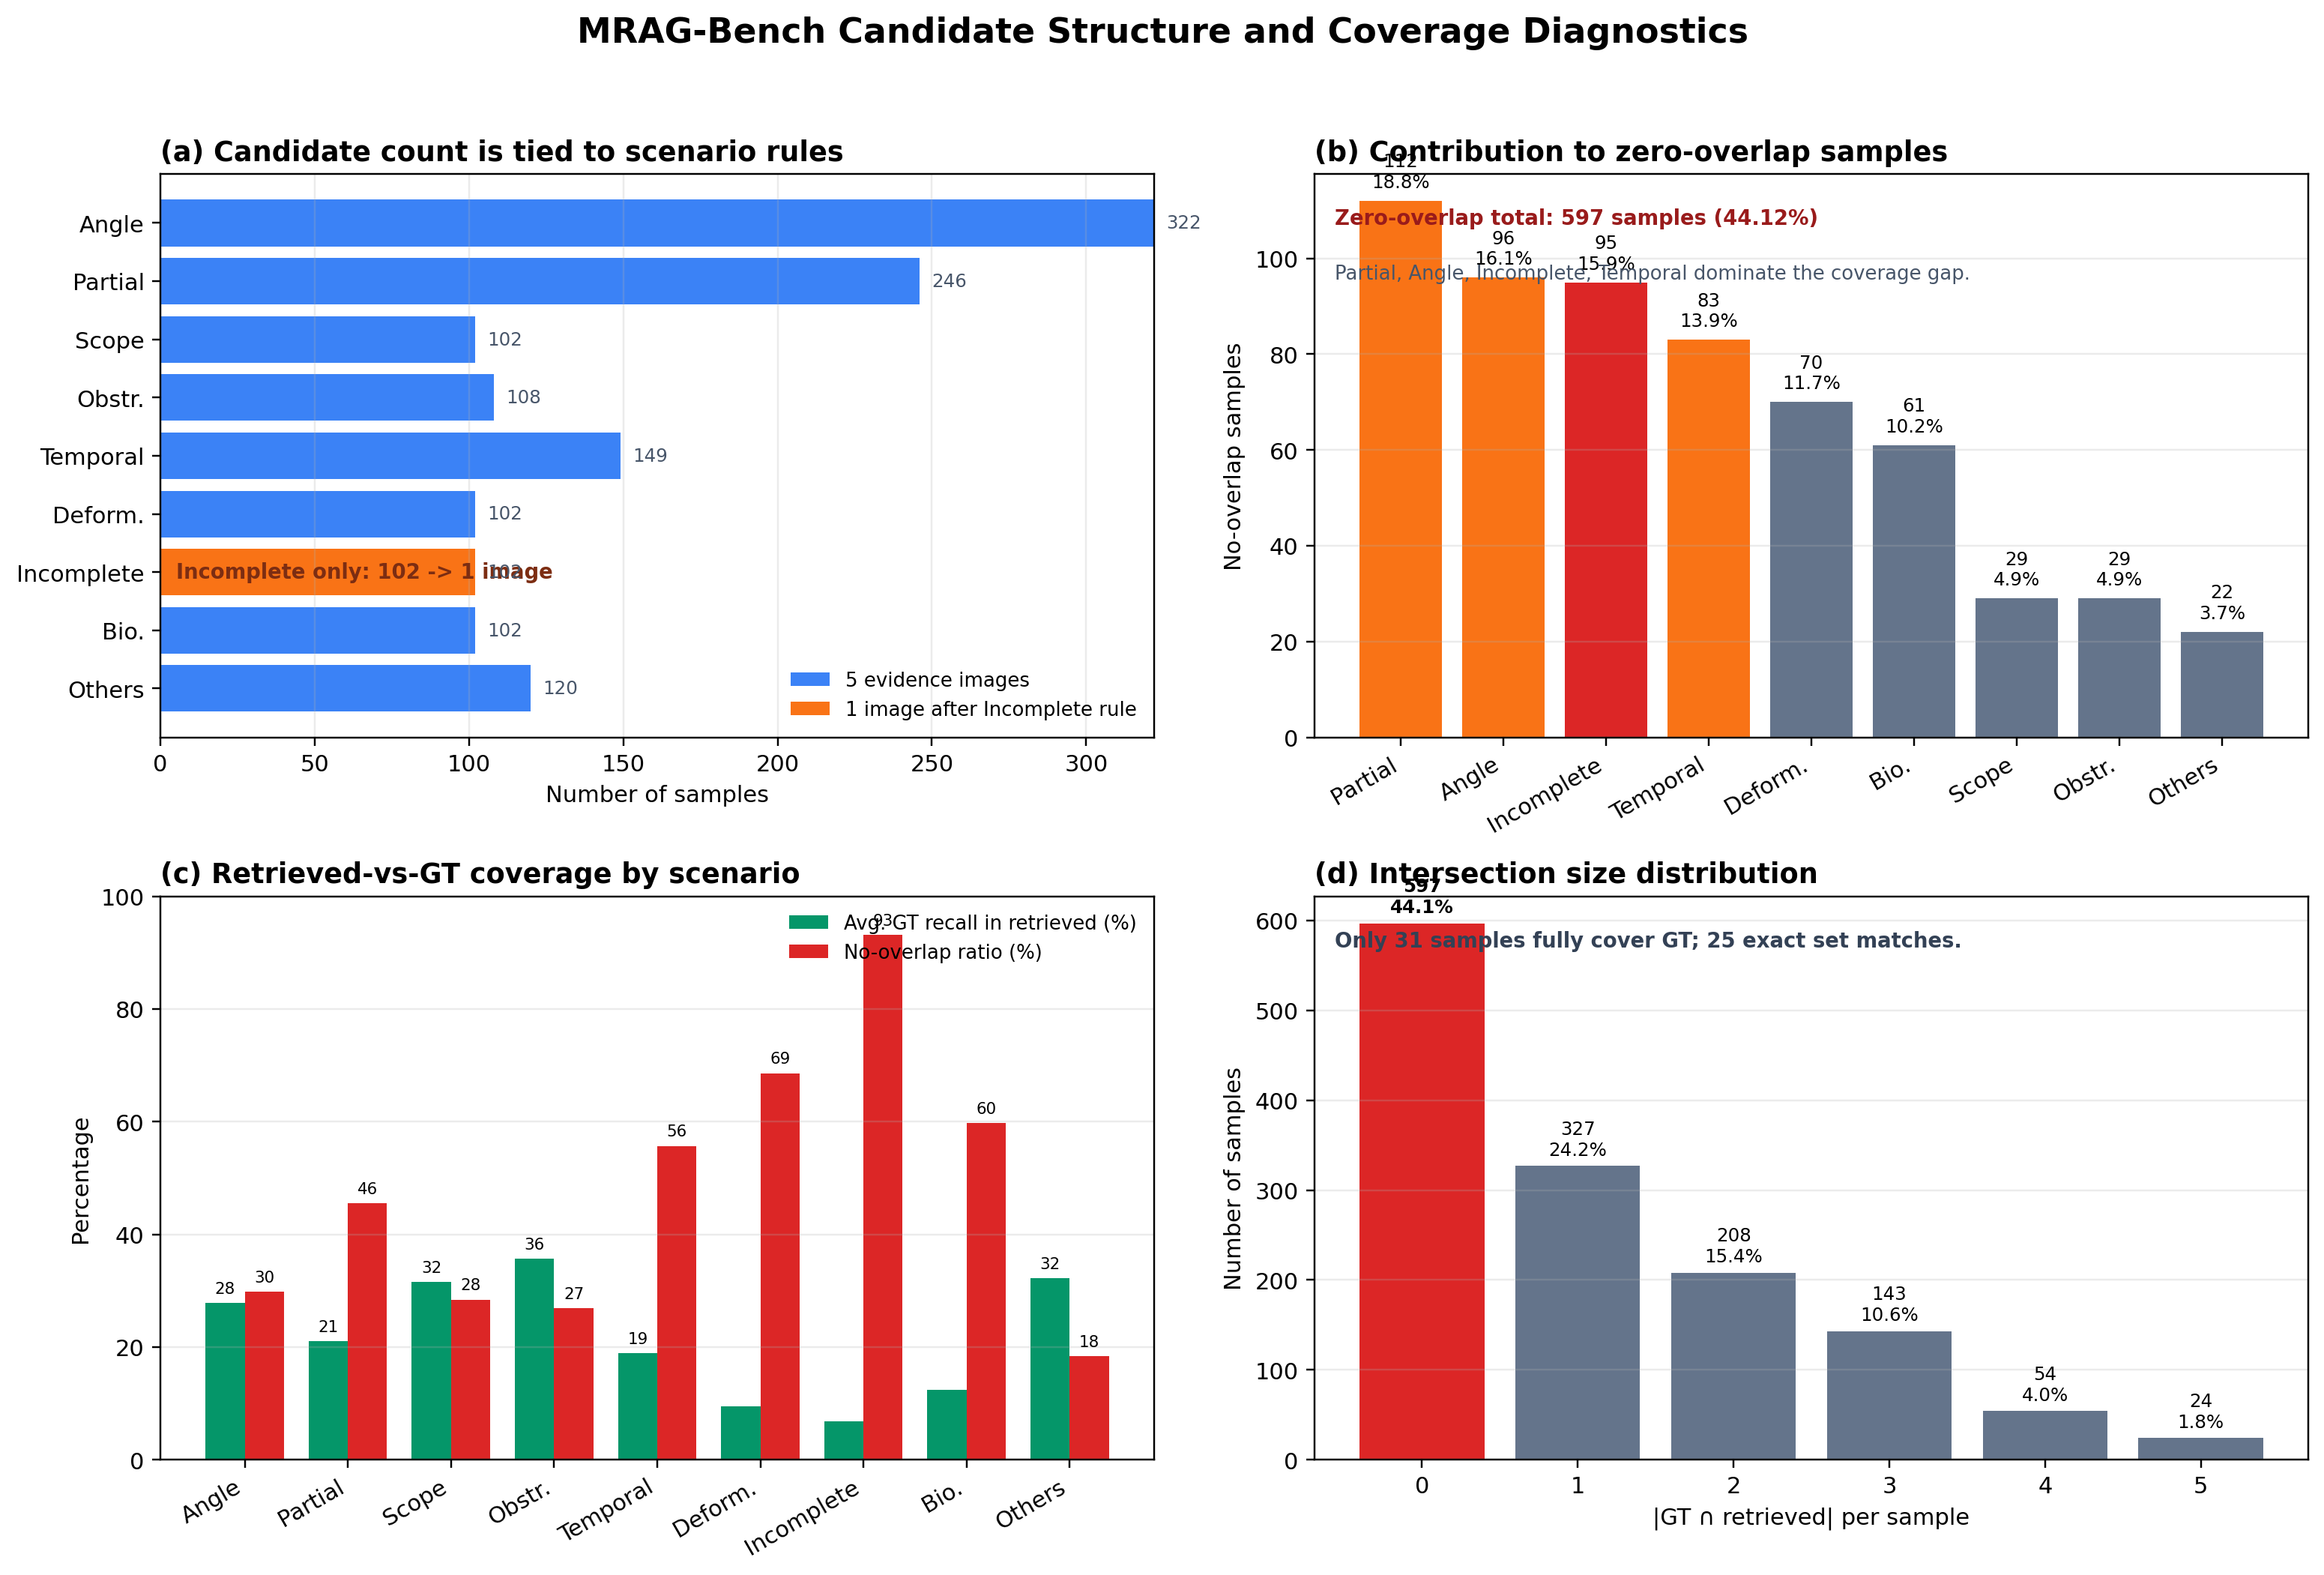
\includegraphics[width=\linewidth]{dataset_candidate_coverage_4panel.png}
\caption{MRAG-Bench 候选覆盖诊断。}
\label{fig:dataset_analysis}
\end{figure}

\section{基于混合检索的多模态生成框架设计}
\label{sec:e8_pipeline}

本文框架把 mRAG 拆成查询构造、候选召回、候选融合和终答生成四个阶段。查询构造阶段负责把原始问题转换为检索器更容易使用的表达；候选召回阶段由 CLIP 或 MagicLens 从外部图像语料库中返回图像候选；候选融合阶段把多路候选压缩为固定长度的证据集合；终答生成阶段则将查询图像、证据图像和原始问题输入 LLaVA-OneVision，并解析最终选项。整个框架固定下游 VLM 和提示模板，把主要变量限制在检索器与查询构造侧。

\subsection{基于通用检索器 CLIP 的检索增强生成框架}

CLIP 分支对应本文中的视觉近邻召回设计。系统首先使用 CLIP ViT-B/32 对完整图像语料库中的每一张图像离线编码，得到可缓存的图像向量索引；推理时，再将样本输入图像编码为 query embedding，并与语料库向量计算相似度，返回 Top-$K$ 候选图像。该分支不使用问题文本进行复杂推理，重点在于建立一个稳定、可扩展、可复现的全库视觉粗召回起点。

从模块职责看，CLIP 不是最终回答模型，也不是关系重排器。它的输入是查询图像与完整图像库，输出是按视觉语义相似度排列的候选图像列表。该设计适合作为混合框架的第一阶段召回器：当查询图像与有效证据在外观或语义上接近时，CLIP 能较快进入相关视觉邻域；当问题需要视角互补、结构补全或细粒度对照时，CLIP 返回的候选则可能需要进一步由关系检索器或查询重写模块处理。

在实现上，CLIP 分支与 MRAG-Bench 原始输入格式解耦。原始评测脚本只负责把既定证据图像交给 VLM，而本文额外实现全库编码、查询向量计算和 Top-$K$ 图像路径回填，使其能够在不依赖 \texttt{retrieved\_images} 字段的情况下自行构造证据集合。

\subsection{基于 MagicLens 的检索增强生成框架}

MagicLens 分支用于建模查询图像、文本指令和目标证据图像之间的关系。与 CLIP 只根据共享向量空间中的视觉语义相似度排序不同，MagicLens 的查询侧同时包含图像和开放式文本指令，因此能够表达“寻找与查询图像满足某种关系的图像”。这使它更适合处理 question-conditioned evidence retrieval，即根据当前问题寻找有用证据，而不是单纯寻找最相似图像。

本文将 MagicLens 放在两类位置上使用。第一类是候选重排：系统先获得一个已有候选集合，再使用 MagicLens 根据查询图像和文本指令对候选重新排序。第二类是直接检索：系统不依赖已有候选字段，而是让 MagicLens 直接在完整图像库上返回候选。二者的区别在于，重排设计受第一阶段候选覆盖限制，而直接检索设计更能体现 MagicLens 自身从全库中组织关系证据的能力。

为了便于与 CLIP 分支对照，MagicLens 输出也被统一整理为 Top-$K$ 图像路径列表，并按同一多图 VQA 输入格式交给下游 LLaVA-OneVision。这样，CLIP 与 MagicLens 在系统层面共享相同的终答入口，差异集中在候选证据的生成方式上。

\subsection{基于 Gemma 4 的多维查询重写与重排序}

单条开放式指令容易遗漏问题中的部分证据需求，也可能过度贴近某个高频视觉模式。为此，本文在 MagicLens 前加入 Gemma~4 查询规划模块，将原始问题拆分为多个互补的检索维度。该分支对应本文主方法 Multi Query RAG(E8)：Gemma~4 读取查询图像、题干和选项，生成 $N$ 条短英文检索指令；MagicLens 按每条指令分别检索；最后通过列表融合得到固定长度的证据集合，再交给 LLaVA-OneVision 终答。图~\ref{fig:arch_baseline_vs_magiclens} 给出了 Multi Query RAG(E8) 的总体流程：系统首先生成五条互补检索指令，随后由 MagicLens 分路检索得到每维 Top-$K$ 候选，多路候选经 RRF 融合为最终 Top-5 视觉证据，最后与问题文本和可选证据描述一同输入 LLaVA-OneVision。该图只描述方法结构，实验结果分析见第 4 章。

\begin{figure}[!htb]
\centering
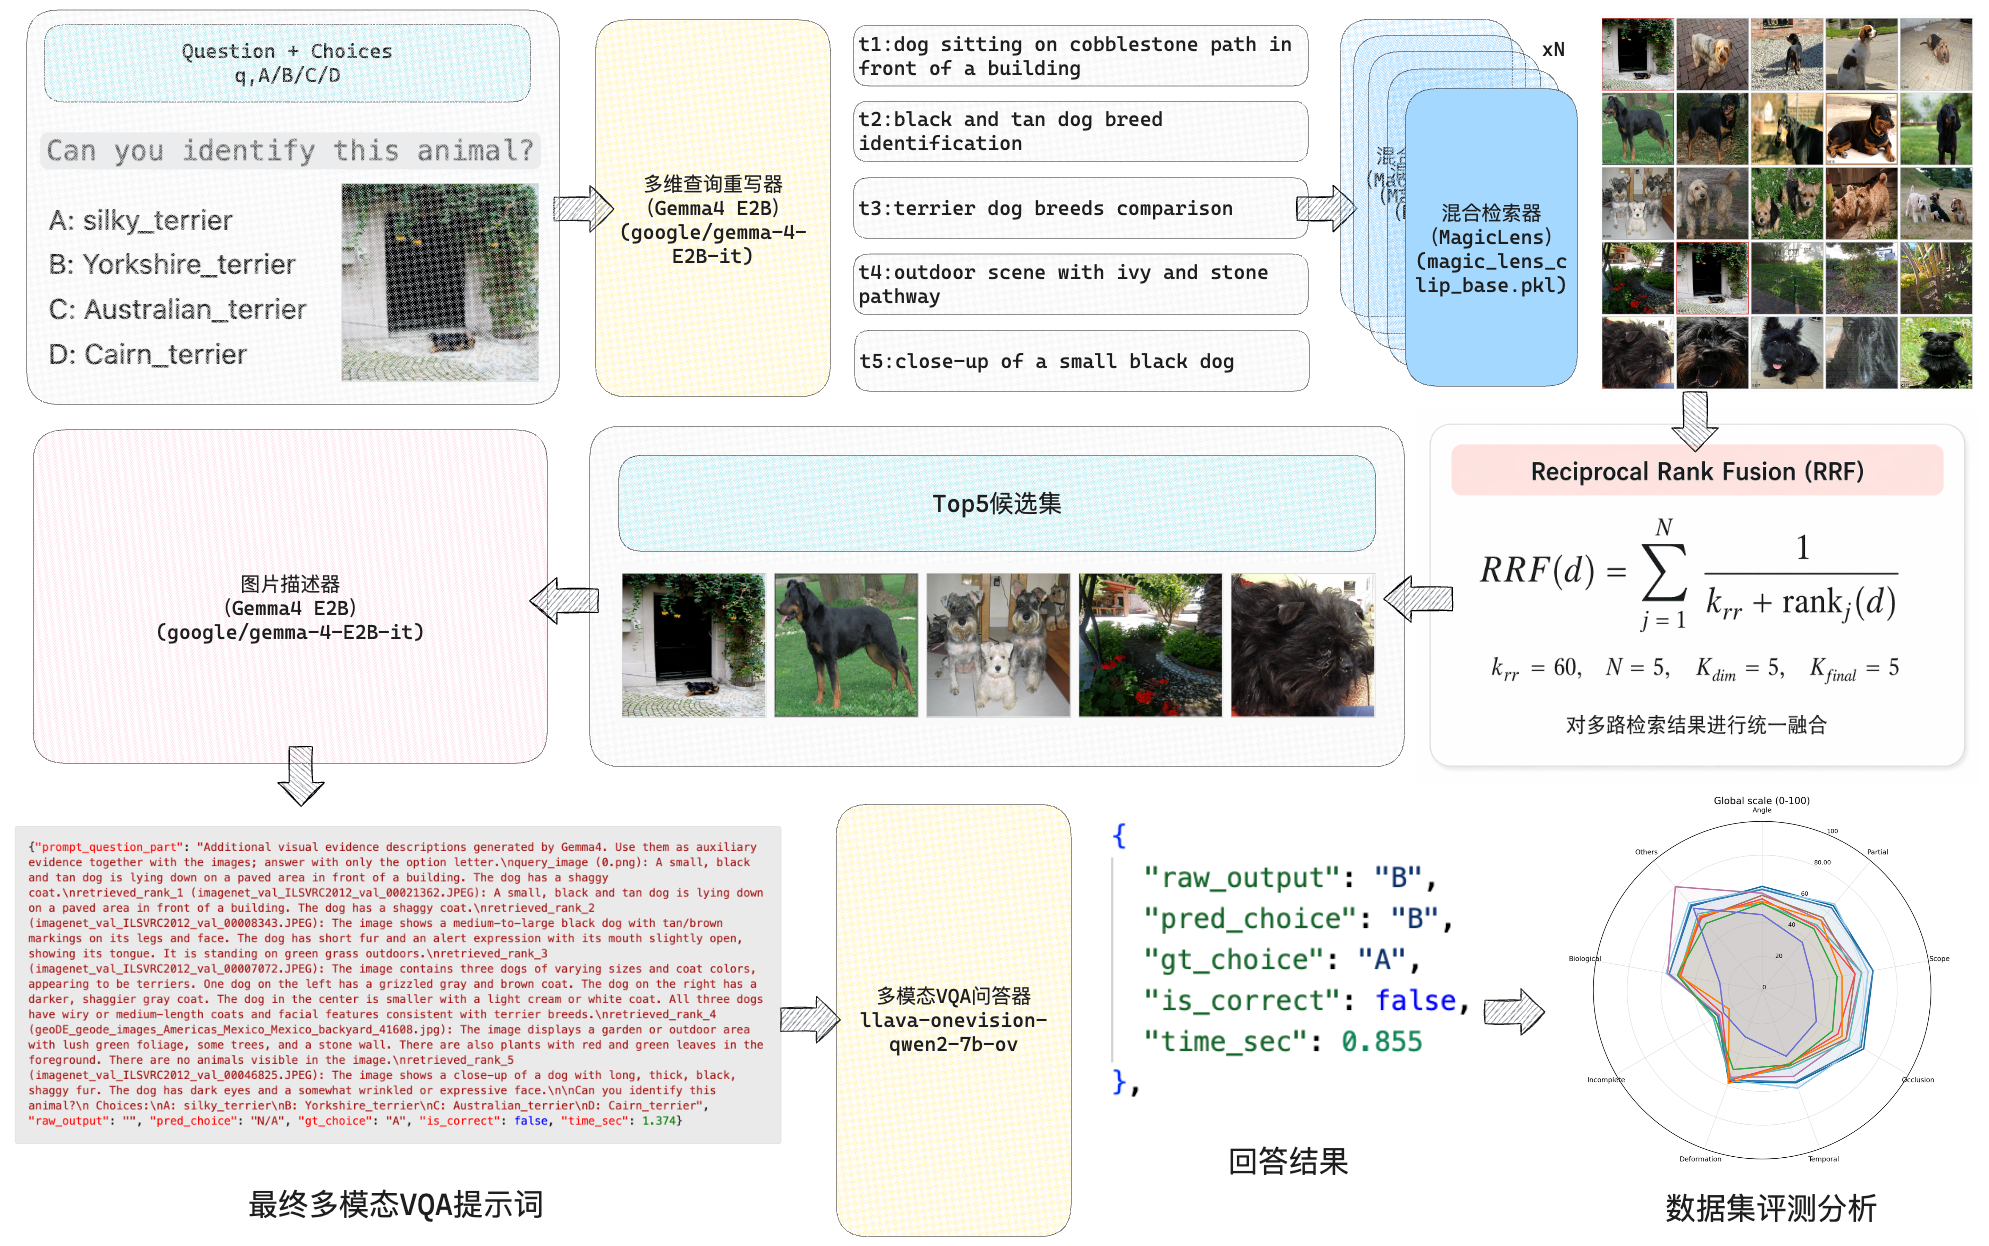
\includegraphics[width=\linewidth]{pipeline_overview.png}
\caption{Multi Query RAG(E8) 框架。}
\label{fig:arch_baseline_vs_magiclens}
\end{figure}

Multi Query RAG(E8) 的一条样本在系统内依次经历维度规划、分路检索、多列表融合、证据描述和多模态终答五个阶段。首先，Gemma~4~E2B-it 读取查询图像与题干，生成 $N$ 条短英文指令，同时输出每条维度的 \texttt{rationale} 作为简短生成理由；检索时只使用 query 字段，不直接拼入 rationale。随后，MagicLens 在查询图像与每条指令的共同条件下，对外部语料分别返回 Top-$K_{\mathrm{dim}}$ 候选列表。系统再对 $N$ 路排序结果做倒数排名和（RRF；本文默认 $K_{\mathrm{rrf}}=60$）或等价的列表融合，得到最终 Top-$K_{\mathrm{final}}$ 证据集合。在终答前，Gemma~4 对“查询图 + 融合后证据图”生成简短自然语言描述，作为 LLaVA 的辅助文本，但不改变图像序列本身。最后，在固定多选项模板下，系统将查询图与选定的融合证据图按约定顺序输入 LLaVA-OneVision，由其输出选项字母，并由下游抽取器解析 A/B/C/D。

上述流程会保存逐样本答案、融合前后检索结果、维度层中间结果以及配套可视化图，包括分维 Top-1 拼图、分维 Top-$K$ 网格、查询图与融合 Top-5 拼图等。过程记录的目的不是在本章讨论得分，而是让系统设计具备可追踪性：如果终答结果不理想，可以进一步检查是维度生成偏离问题、某一路检索返回噪声，还是融合后证据集合没有覆盖关键视觉条件。

由于 MRAG-Bench 中检索候选主要以图像路径形式存在，缺少能够直接描述候选证据内容的文本字段，本文在 Multi Query RAG(E8) 中额外加入证据描述补充步骤：由 Gemma~4 对查询图像与融合后候选图像生成简短文本描述，再将这些描述作为辅助信息拼入终答提示词。该步骤不训练新的检索器，而是在固定模型参数的推理流程中补足候选图像的显式语义信息，使下游 VLM 能够同时利用图像输入和文本化证据摘要。

Multi Query RAG(E8) 在“查询链 + 全库多模态 RAG”意义上的方法扩展主要体现在四个方面。其一是多视角指令规划，即在查询图像与题干共同约束下生成互补检索子任务，降低单条指令过度贴近某一外观模式导致的排序偏置。其二是多路可融合排序，即在 MagicLens 返回的多份候选列表上引入显式融合算子，使不同语义维度的证据能够在排序层面被折中整合。其三是推理期扩展且无需更新检索器参数，维数、每维 Top-$K$、融合策略与终答用图数均可在配置层调整，与本文强调的 inference-time 方法路线一致。其四是 VLM 下的端到端可对照，即在 LLaVA 与提示模板的框架内，将改进集中在检索前端的查询与融合设计，使对比结论可解释、可复现。

为了进一步说明 Multi Query RAG(E8) 并非停留在概念流程，而是一个可执行、可检查的推理管线，下面给出其伪代码描述。该描述突出系统在单个样本上的实际执行顺序，以及每一步需要记录的中间状态。

\begin{center}
\setlength{\fboxsep}{5pt}
\fbox{%
\begin{minipage}{0.94\linewidth}
\footnotesize
\noindent\textbf{算法 3-1：Multi Query RAG(E8) 多维检索式 RAG 推理过程}
\vspace{0.2em}
\hrule
\vspace{0.25em}
\noindent\textbf{输入：} 查询图像 $I_q$，问题 $Q$，选项集合 $C=\{A,B,C,D\}$，图像语料库 $\mathcal{D}$。\\
\textbf{输出：} 最终答案选项 $\hat{y}\in\{A,B,C,D\}$。\\
\textbf{参数：} 维度数 $N=5$，每维召回数 $K_{\mathrm{dim}}=5$，最终证据数 $K_{\mathrm{final}}=5$，RRF 平滑常数 $K_{\mathrm{rrf}}=60$。
\vspace{0.25em}
\hrule
\vspace{0.2em}

\noindent\textbf{Step 1.} 将 $I_q$、$Q$ 与 $C$ 输入 Gemma~4，生成 $N$ 条互补的英文检索指令 $\{q_1,q_2,\ldots,q_N\}$，并记录每条指令对应的生成理由。\par
\vspace{0.1em}
\noindent\textbf{Step 2.} 对于每条检索指令 $q_i$，将 $(I_q,q_i)$ 输入 MagicLens，在完整语料库 $\mathcal{D}$ 中检索 Top-$K_{\mathrm{dim}}$ 候选图像，得到排序列表 $R_i$。\par
\vspace{0.1em}
\noindent\textbf{Step 3.} 合并 $N$ 个排序列表。对于候选图像 $d$，按
\[
S(d)=\sum_{i=1}^{N}\frac{1}{K_{\mathrm{rrf}}+\mathrm{rank}_i(d)}
\]
计算融合得分；若 $d$ 未出现在第 $i$ 路结果中，则该路不贡献得分。\par
\vspace{0.1em}
\noindent\textbf{Step 4.} 按 $S(d)$ 从高到低排序，取前 $K_{\mathrm{final}}$ 张图像作为最终证据集合 $E$。\par
\vspace{0.1em}
\noindent\textbf{Step 5.} 使用 Gemma~4 对查询图像和最终证据图像生成简短证据描述，形成面向终答模型的辅助文本。\par
\vspace{0.1em}
\noindent\textbf{Step 6.} 构造终答提示词：包括原始问题 $Q$、选项集合 $C$、查询图像 $I_q$、最终证据集合 $E$ 以及证据描述。\par
\vspace{0.1em}
\noindent\textbf{Step 7.} 将上述多模态输入送入 LLaVA-OneVision，得到原始回答文本 $o$。\par
\vspace{0.1em}
\noindent\textbf{Step 8.} 从 $o$ 中解析选项字母，得到最终预测 $\hat{y}$；同时记录每维 Top-$K$、融合 Top-5、终答提示词、原始输出、解析选项和各阶段耗时。\par

\vspace{0.1em}
\hrule
\vspace{0.2em}
\noindent\textbf{运行设置：} 推理阶段不更新 Gemma~4、MagicLens 或 LLaVA-OneVision 的参数；单样本串行执行，VLM 生成阶段 batch size 为 1；Gemma~4 与 LLaVA-OneVision 使用 GPU 推理，MagicLens 在本文正式 Multi Query RAG(E8) 运行中采用 CPU 后端完成检索。
\end{minipage}%
}
\end{center}

\section{多维查询分析}


\label{sec:e8_example_qs0}

为了更具体地说明多维查询在单个样本上是如何展开的，这里选取样本 \texttt{qs\_id=0} 作为示例。该样本能够体现 Multi Query RAG(E8) 的一个关键特点，即系统并不把问题压缩为单一检索指令，而是将其拆分为若干相互补充的检索目标。表~\ref{tab:e8_qs0_dims} 列出了该样本生成的五条检索子任务及其对应的生成依据，用于展示系统如何从原始问题中提炼出主体识别、局部细节、背景关系和相似候选等不同方向的检索需求。

\begin{table}[!htb]
\centering
\scriptsize
\caption{Multi Query RAG(E8) 样例 \texttt{qs\_id=0}：多维度查询指令与生成理由。}
\label{tab:e8_qs0_dims}
\resizebox{\textwidth}{!}{%
\begin{tabular}{clp{9.5cm}}
\toprule
\textbf{维} & \textbf{query（用于 MagicLens 检索，与 rationale 解耦）} & \textbf{rationale（生成该查询的简短理由）} \\
\midrule
1 & \texttt{dog sitting on cobblestone path in front of a building} & This focuses on identifying the main subject, the dog, in its environment. \\
2 & \texttt{black and tan dog breed identification} & This aims to get breed-specific information about the dog's appearance. \\
3 & \texttt{terrier dog breeds comparison} & This helps narrow down the options by focusing on the category of dogs presented. \\
4 & \texttt{outdoor scene with ivy and stone pathway} & This captures the background context, which might offer clues about the location or style. \\
5 & \texttt{close-up of a small black dog} & A close-up might reveal finer details of the dog's coat and features. \\
\bottomrule
\end{tabular}%
}
\end{table}

多路结果经 RRF 融合后，得到长度 $K_{\mathrm{final}}=5$ 的候选集；其倒数排名和形式为
\begin{equation}
\mathrm{RRF}(d)=\sum_{j=1}^{N}\frac{1}{K_{\mathrm{rrf}}+\mathrm{rank}_j(d)},
\end{equation}
其中 $\mathrm{rank}_j(d)$ 为第 $j$ 条指令对应列表中候选项 $d$ 的名次，若 $d$ 未出现则不计入。

在终答阶段，系统向 LLaVA 提供的文本为固定模板下的多选项问题，并附加 Gemma~4 生成的证据图描述作为辅助。代码片段 3-1 给出生成日志中的 \texttt{prompt\_question\_part} 片段（英文原文；描述文本略去部分换行以节省版面）：

\begin{figure}[!htbp]
\centering
\fbox{%
\begin{minipage}{0.94\linewidth}
\footnotesize
\noindent\textbf{代码片段 3-1：\texttt{prompt\_question\_part} 终答提示片段}
\vspace{0.2em}
\hrule
\vspace{0.25em}
\ttfamily
\setlength{\parindent}{0pt}
Additional visual evidence descriptions generated by Gemma4. Use them\par
as auxiliary evidence together with the images; answer with only\par
the option letter.\par
query\_image (0.png): A small, black and tan dog is lying down ...\par
... (retrieved\_rank\_1..5 descriptions) ...\par
Can you identify this animal?\par
\ Choices:\par
A: silky\_terrier\par
B: Yorkshire\_terrier\par
C: Australian\_terrier\par
D: Cairn\_terrier\par
\end{minipage}%
}
\end{figure}

仅列出检索子任务还不足以说明多维查询为何可能有效，还需要进一步看到这些子任务各自召回了什么图像、不同维度之间是否出现重复命中，以及融合后的最终证据集合与原查询图之间形成了怎样的对应关系。基于这一目的，图~\ref{fig:e8_qs0_viz} 将该样例展开为三类可视化结果：\textbf{(a)}~各维度 Top-1 的横向拼贴，用于观察不同维度最先命中的证据类型；\textbf{(b)}~“维度 $\times$ 名次”的网格总览，用于比较跨维重复命中与排序结构；\textbf{(c)}~查询图与融合后 Top-5 证据的拼图，用于展示最终送入多模态终答模型的图像条件。

\begin{figure}[!htbp]
\centering
\captionsetup{aboveskip=0.25\baselineskip,belowskip=0.35\baselineskip}
\captionsetup[subfigure]{aboveskip=0.15\baselineskip,belowskip=0.15\baselineskip}
\begin{subfigure}{0.92\linewidth}
    \centering
    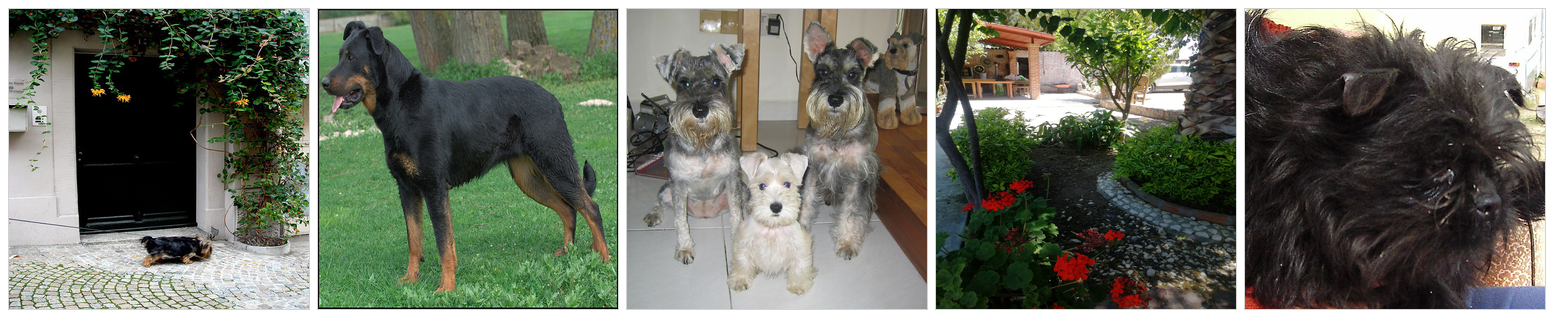
\includegraphics[width=\linewidth]{e8_qs0_dim_top1_1x5.png}
    \caption{各检索维度的 Top-1 候选。}
\end{subfigure}\\[-0.15em]
\begin{subfigure}{0.92\linewidth}
    \centering
    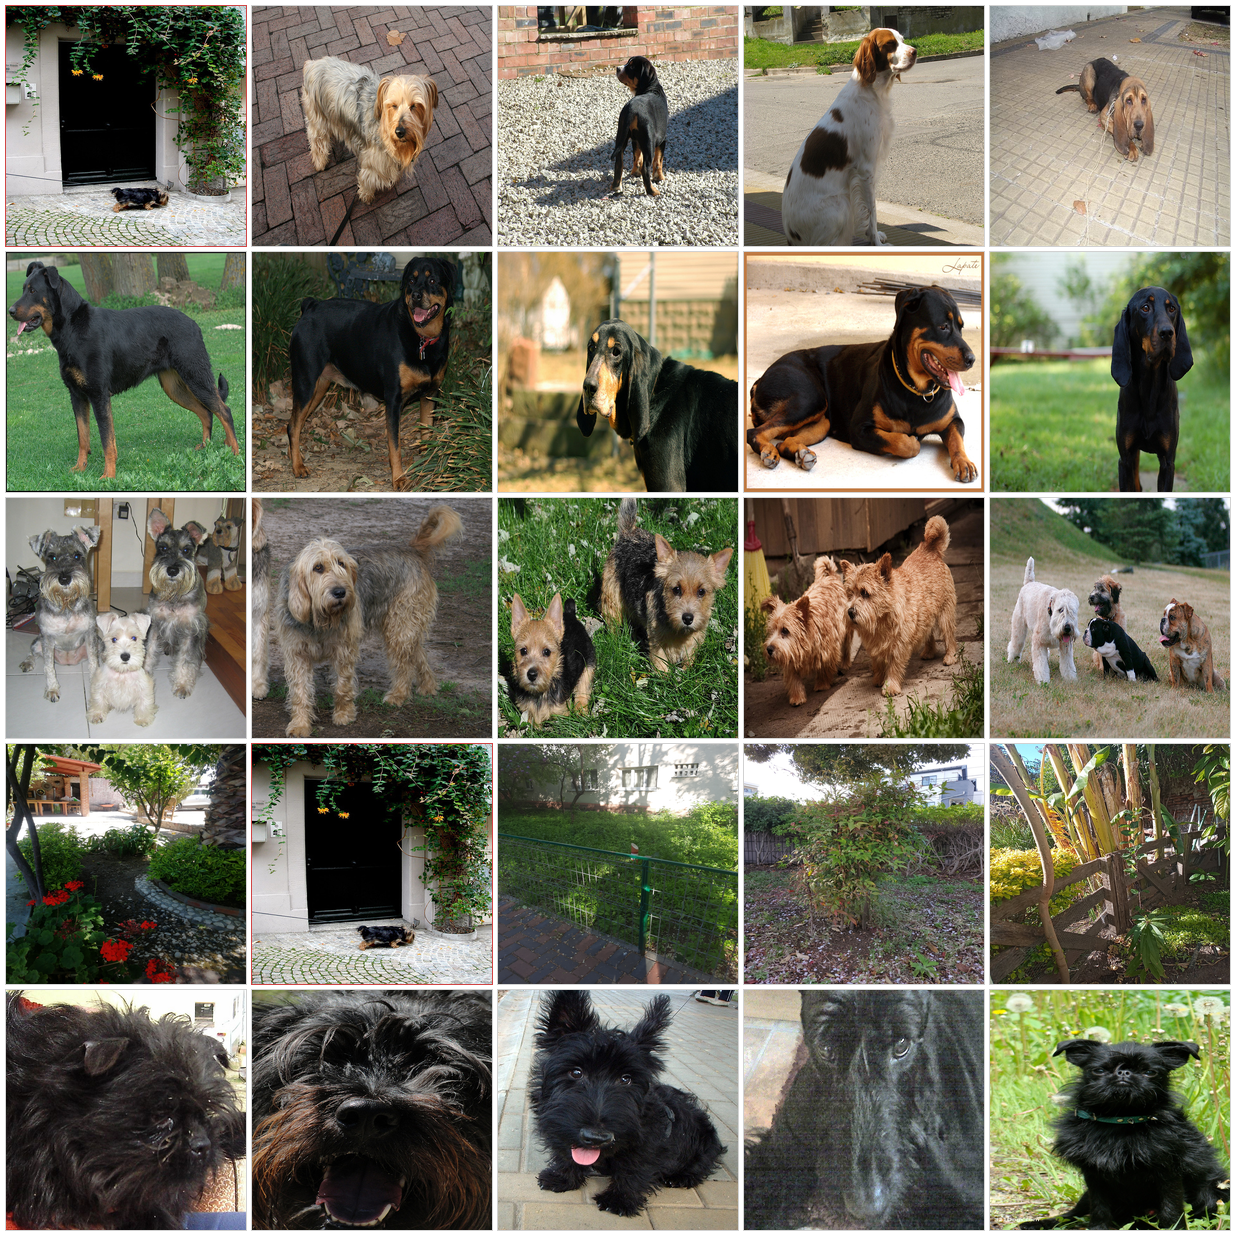
\includegraphics[width=\linewidth]{e8_qs0_dim_topk_grid.png}
    \caption{维度 $\times$ 排名的 Top-$K$ 候选网格。}
\end{subfigure}\\[-0.15em]
\begin{subfigure}{0.92\linewidth}
    \centering
    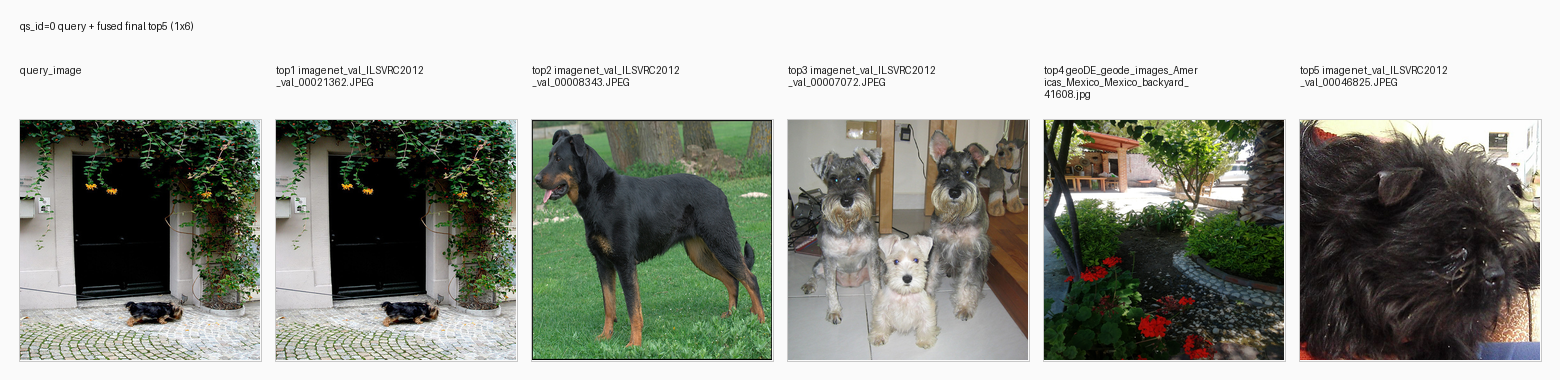
\includegraphics[width=\linewidth]{e8_qs0_query_plus_final_top5_1x6.png}
    \caption{查询图与 RRF 融合后的最终 Top-5 证据。}
\end{subfigure}
\caption{Multi Query RAG(E8) 样例检索可视化。}
\label{fig:e8_qs0_viz}
\end{figure}

该样例展示的是 Multi Query RAG(E8) 的设计过程，而不是模型得分。结合图~\ref{fig:e8_qs0_viz} 可以看到，多维查询使同一问题被拆成多个检索视角：有的维度关注主体类别，有的维度关注背景环境，有的维度强调局部外观。最终进入 LLaVA 的不是某一路检索的原始输出，而是经过 RRF 融合后的证据集合。这种过程性可视化有助于检查多维查询是否真正扩大了证据搜索空间，以及融合结果是否仍保留了与原问题相关的视觉条件。


\chapter{实验结果分析}

\section{实验设置}

为了验证第 3 章提出的混合检索式 mRAG 框架是否有效，本文围绕四类问题组织实验：第一，进行上限探究实验，观察人工证据条件下系统能够达到的参考水平；第二，进行对比实验，将本文方法与 CLIP、MagicLens 及其组合进行比较；第三，进行消融实验，分析查询重写、终答器等关键模块的作用；第四，进行参数概述实验，说明多维查询数量、每维候选数和融合策略等设置对系统行为的影响。本章只讨论实验结果与机制解释，方法结构已在第 3 章给出。

\subsection{数据集划分}

本文实验使用 MRAG-Bench 的 test split，共 1353 个样本和 16130 张图像。数据集按场景划分为九类：\textit{Angle}、\textit{Partial}、\textit{Scope}、\textit{Occlusion/Obstruction}、\textit{Temporal}、\textit{Deformation}、\textit{Incomplete}、\textit{Biological} 与 \textit{Others}。主实验、上限实验、对比实验与主要消融实验均在完整 test split 上运行；参数选择阶段受计算成本限制，不对所有参数组合做全量穷举，而以已完成的全量配置和候选结构统计作为正文依据。

\subsection{评价指标}

本文采用整体准确率（Overall Accuracy）和分场景准确率（Scenario Accuracy）评估最终多选题作答结果。为了进一步解释检索阶段本身，本文同时统计证据召回率：Recall@5 表示最终进入终答阶段的 Top-5 图像是否覆盖人工 GT 证据，Recall@N 表示融合前候选池是否覆盖 GT 证据。对于检索器差异，本文还使用 Top-5 overlap、Top-1 match rate、逐样本胜负统计和高频重复命中分布等指标分析候选结构。对于系统效率，本文统计单样本总耗时及维度规划、检索融合、证据描述、终答生成等模块的耗时。

\subsection{结果总览}

表~\ref{tab:exp2_real_rag} 汇总了 GT RAG(E0) 至 Raw Query(E10) 的整体结果与分场景表现。表中 GT RAG(E0)、GT Rerank(E1)、GT Direct(E5) 属于人工证据参考设置，用于探索框架上限；Retrieved Rerank(E2) 表示在数据集给定 retrieved candidates 上使用 MagicLens 重排；CLIP Retrieval(E3)、CLIP Rerank(E6)、MagicLens Retrieval(E7) 是完整 corpus 检索对比基线；No RAG(E4) 表示 LLaVA 不使用外部证据；Multi Query RAG(E8) 是本文主框架；Gemma Answerer(E9) 和 Raw Query(E10) 分别用于终答器替换和查询重写消融。颜色仅用于辅助阅读：绿色表示人工证据参考设置，红色表示完整 corpus 检索基线，蓝色表示本文主框架及关键能力对比项。

\begin{table}[!htb]
\centering
\scriptsize
\caption{实验命名与结果总表。}
\label{tab:exp2_real_rag}
\resizebox{\textwidth}{!}{
\begin{tabular}{l c c c c c c c c c c}
\toprule
\multirow{2}{*}{Method} & \multirow{2}{*}{Overall}
& \multicolumn{4}{c}{Perspective}
& \multicolumn{4}{c}{Transformative}
& \multirow{2}{*}{Others} \\
\cmidrule(lr){3-6} \cmidrule(lr){7-10}
&
& Angle & Partial & Scope & Obstruction
& Temporal & Deformation & Incomplete & Biological \\
\midrule
\upperbase{GT RAG(E0)} & 59.05 & 59.63 & 64.23 & 66.67 & 67.59 & 57.72 & 56.86 & 29.41 & 55.88 & 64.17 \\
\upperbase{GT Rerank(E1)} & 60.16 & 61.49 & 65.45 & 66.67 & 69.44 & 58.39 & 57.84 & 30.39 & 55.88 & 65.00 \\
Retrieved Rerank(E2) & 51.74 & \secondworst{51.24} & 50.41 & \secondbest{59.80} & \best{59.26} & 48.99 & 55.88 & \best{33.33} & 50.00 & 59.17 \\
\lowerbase{CLIP Retrieval(E3)} & 50.41 & 52.48 & \secondbest{54.07} & 48.04 & 54.63 & \secondworst{46.31} & \best{58.82} & \worst{22.55} & 50.00 & 57.50 \\
\upperbase{No RAG(E4)} & 53.14 & \secondbest{56.21} & \best{56.10} & 55.88 & \secondbest{57.41} & 47.65 & 55.88 & \best{33.33} & \secondbest{50.98} & \secondworst{55.83} \\
\upperbase{GT Direct(E5)} & 60.16 & 59.94 & 66.67 & 63.73 & 66.67 & 61.74 & 56.86 & 29.41 & 57.84 & 67.50 \\
CLIP Rerank(E6) & 50.33 & 54.04 & 49.19 & 55.88 & 51.85 & \secondworst{46.31} & \secondbest{56.86} & 27.45 & \secondworst{49.02} & 56.67 \\
\lowerbase{MagicLens Retrieval(E7)} & \secondworst{47.97} & 51.55 & \secondworst{47.56} & \secondworst{45.10} & \secondworst{48.15} & 46.98 & \secondworst{50.00} & \secondbest{32.35} & \secondbest{50.98} & \worst{51.67} \\
\modelcap{Multi Query RAG(E8)} & 56.32 & 57.45 & \secondbest{54.07} & 59.80 & \secondbest{57.41} & 54.36 & 54.90 & 29.41 & \worst{25.49} & \secondbest{80.00} \\
\modelcap{Optimized Multi Query RAG(E11\_4)} & \best{57.43} & 59.32 & 54.88 & \best{62.75} & 55.56 & 57.05 & 50.98 & 31.37 & 55.88 & \best{84.17} \\
\modelcap{Gemma Answerer(E9)} & \worst{38.95} & \worst{44.72} & \worst{36.99} & \worst{30.39} & \worst{37.04} & \worst{41.61} & \worst{29.41} & 26.47 & \worst{25.49} & \secondbest{63.33} \\
Raw Query(E10) & \secondbest{53.51} & 54.66 & 50.81 & \best{61.76} & 56.48 & \best{57.72} & 53.92 & \secondworst{24.51} & \best{57.84} & 61.67 \\
\bottomrule
\end{tabular}
}
\end{table}

\section{框架性能理论上限探索}

上限探究实验用于回答一个基础问题：如果系统已经获得人工标注的有效证据，下游多模态模型能够达到什么水平。本文使用 GT RAG(E0)、GT Rerank(E1) 和 GT Direct(E5) 作为上限参考。GT RAG(E0) 直接使用 GT 证据作答，GT Rerank(E1) 在 GT 证据上加入 MagicLens 重排，GT Direct(E5) 则直接使用 GT 证据且不重排。它们并不代表真实全库检索能力，而是用于估计“证据已经足够好”时框架的理论参考上限。

从整体结果看，GT Direct(E5) 的整体准确率为 \best{60.16\%}，GT Rerank(E1) 同样达到 \best{60.16\%}，GT RAG(E0) 为 59.05\%。这说明在人工证据条件下，下游 VLM 能较稳定地利用视觉证据作答；同时，GT 候选上的重排并未带来显著额外收益，系统瓶颈更可能来自候选覆盖与多图证据利用，而不是简单排序。作为对照，No RAG(E4) 的整体准确率为 \focusval{53.14\%}，说明外部证据只有在质量较高时才会稳定带来收益。

图~\ref{fig:overall_and_control_compare} 从整体准确率和控制组角度展示这一关系。人工证据相关设置位于整体结果前列，而真实全库检索基线 CLIP Retrieval(E3)、CLIP Rerank(E6)、MagicLens Retrieval(E7) 与人工证据参考设置之间仍存在明显差距。图中同时纳入 Multi Query RAG(E8)、Optimized Multi Query RAG(E11\_4)、Gemma Answerer(E9) 和 Raw Query(E10)，用于对照主方法、参数优化与关键消融设置。这个差距就是本文后续混合检索框架需要缩小的空间。

\begin{figure}[!htb]
\centering
\begin{subfigure}{0.48\linewidth}
    \centering
    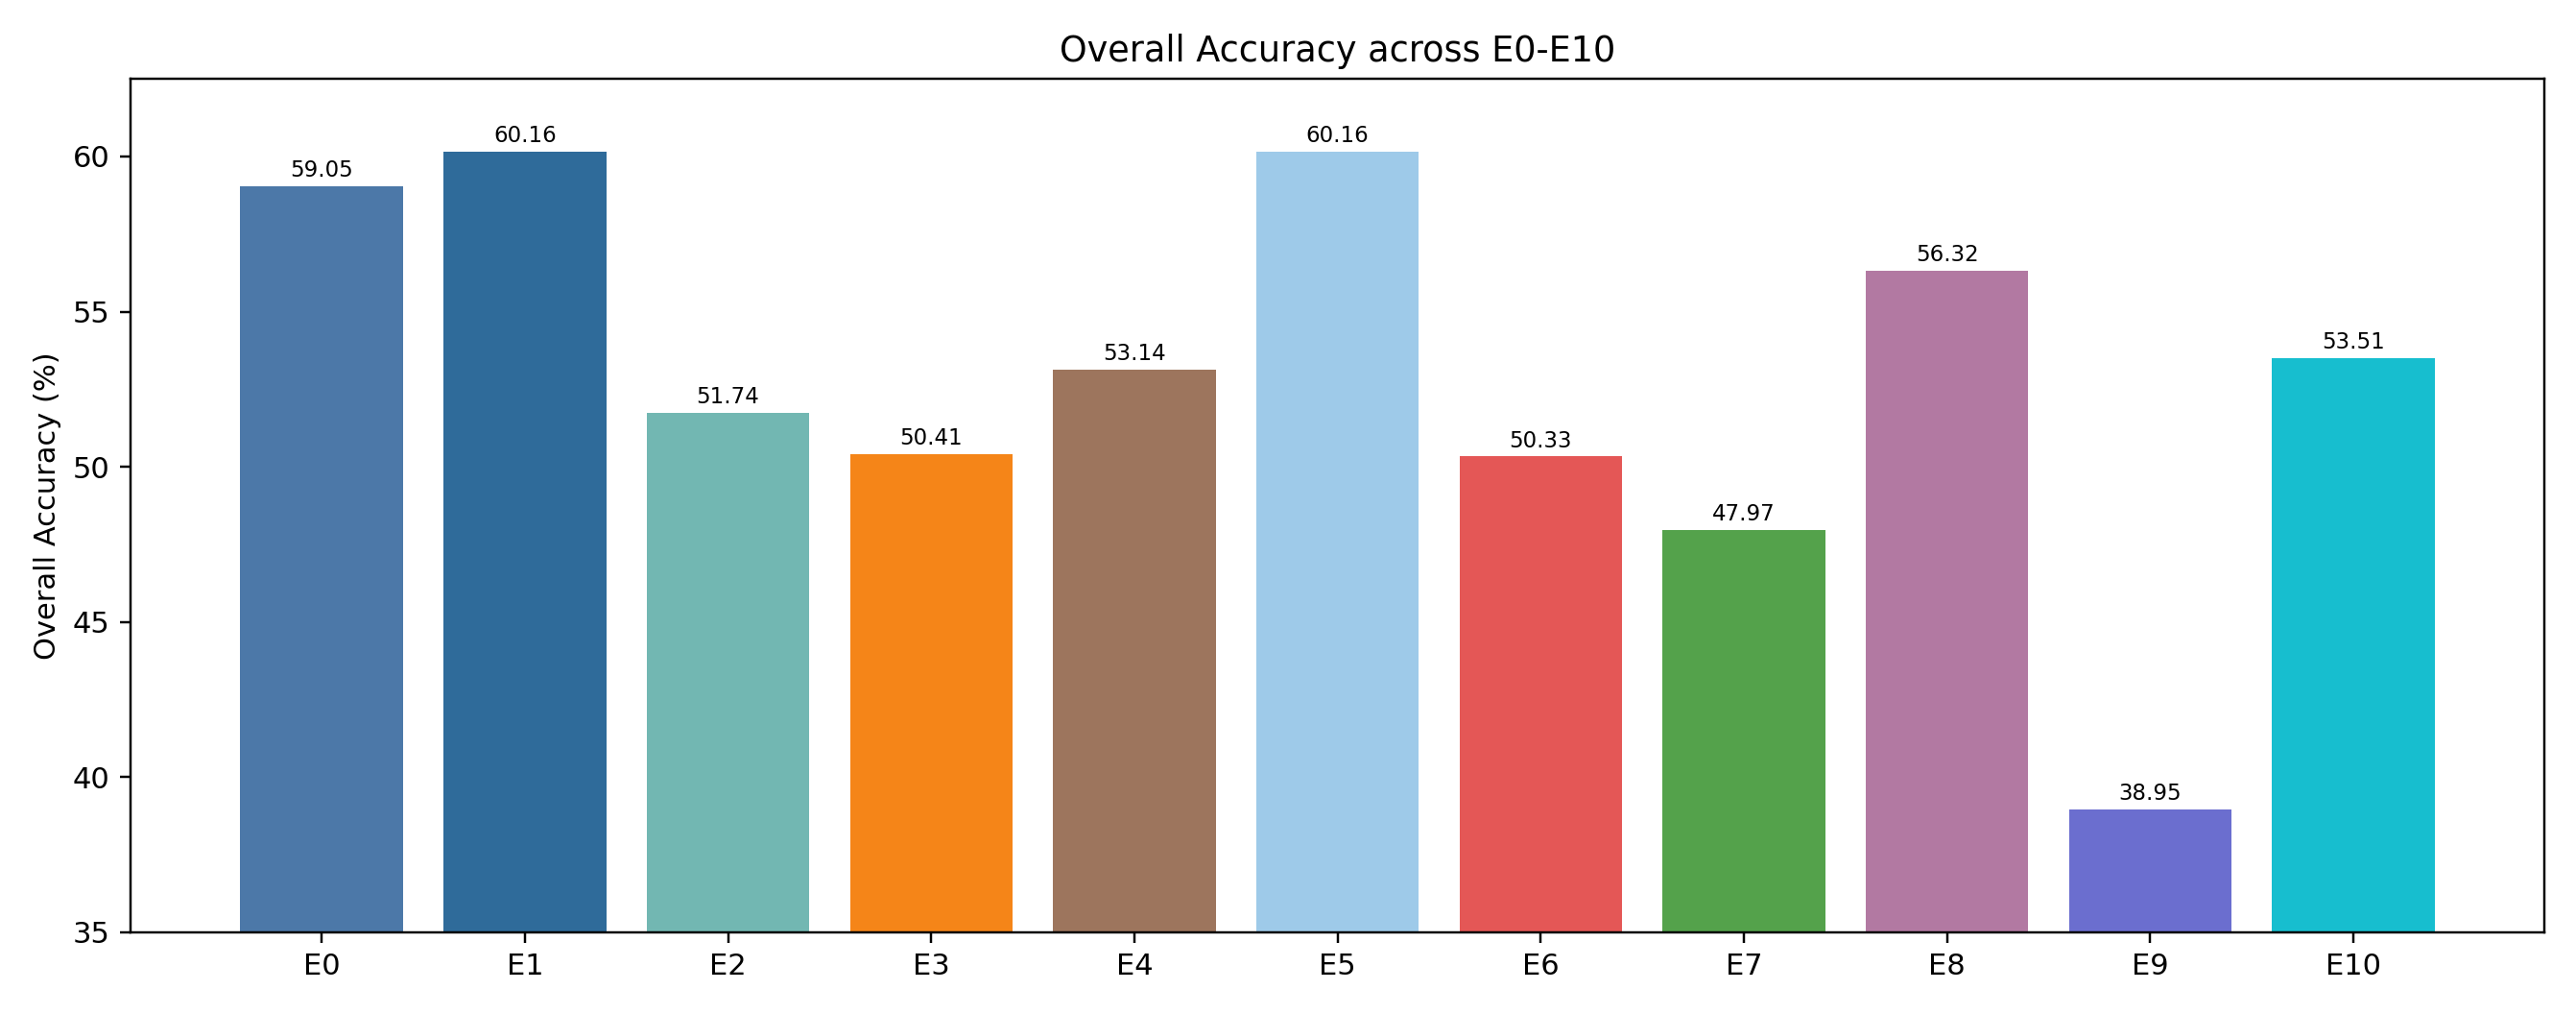
\includegraphics[width=\linewidth]{overall_accuracy_e0_e10.png}
    \caption{整体准确率对比。}
\end{subfigure}
\hfill
\begin{subfigure}{0.48\linewidth}
    \centering
    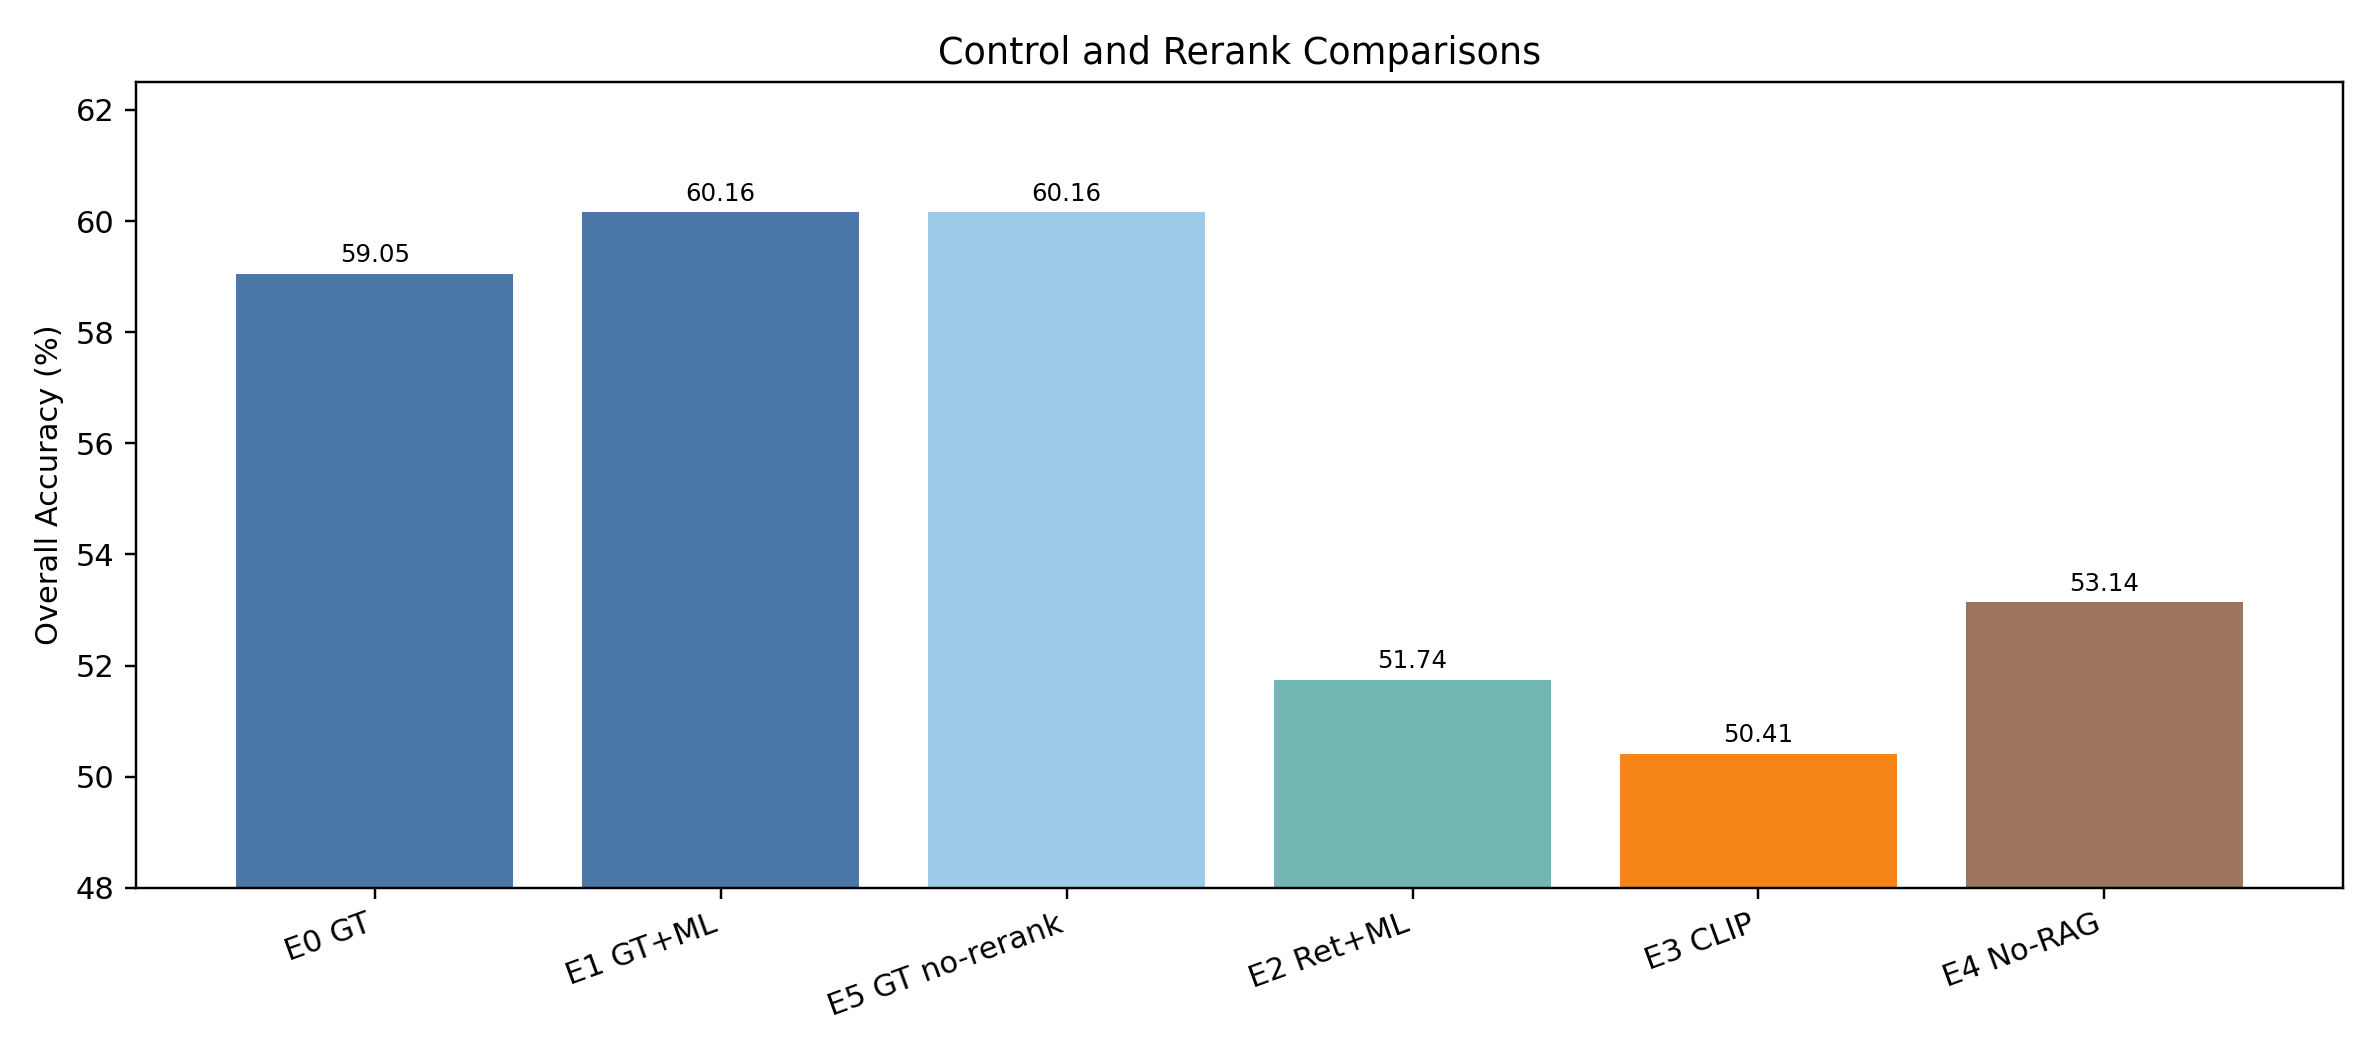
\includegraphics[width=\linewidth]{control_rerank_compare.png}
    \caption{控制实验与 rerank 对照结果。}
\end{subfigure}
\caption{总体准确率与证据条件上限。}
\label{fig:overall_and_control_compare}
\end{figure}

\section{对比实验结果与时间效率分析}

\subsection{本文多维融合框架的整体表现}

Multi Query RAG(E8) 是本文主框架的初始配置：Gemma~4 生成五维查询，MagicLens 分路检索，RRF 融合候选，再由 LLaVA-OneVision 终答。它在完整 test split 上达到 56.32\%，显著高于 CLIP Retrieval(E3) 的 50.41\%、CLIP Rerank(E6) 的 50.33\% 和 MagicLens Retrieval(E7) 的 47.97\%。在此基础上，Optimized Multi Query RAG(E11\_4) 将查询维度数从 5 减少到 4，并保持每维 Top-5、最终 Top-5 与 RRF 融合不变，最终达到 57.43\%。这说明单一检索器或简单重排不足以稳定解决完整图像库检索问题，而查询侧多维规划与列表融合可以改善非人工证据条件下的系统表现；同时，多维查询也不是维度越多越好，适当减少噪声维度可以进一步提升性能。

仅看准确率仍然不够，因为答错并不一定意味着检索失败，也可能是终答阶段未能充分利用已有证据。因此，图~\ref{fig:e0_e13_recall} 从证据召回率角度补充分析。Multi Query RAG(E8) 的最终 Recall@5 为 5.42\%，但融合前候选池 Recall@N 达到 14.13\%，明显高于 MagicLens Retrieval(E7) 单路直检。这说明多维查询真正扩大的主要是融合前的有效证据覆盖范围，而最终 Top-5 的压缩仍会带来一定信息损失。

\begin{figure}[!htb]
\centering
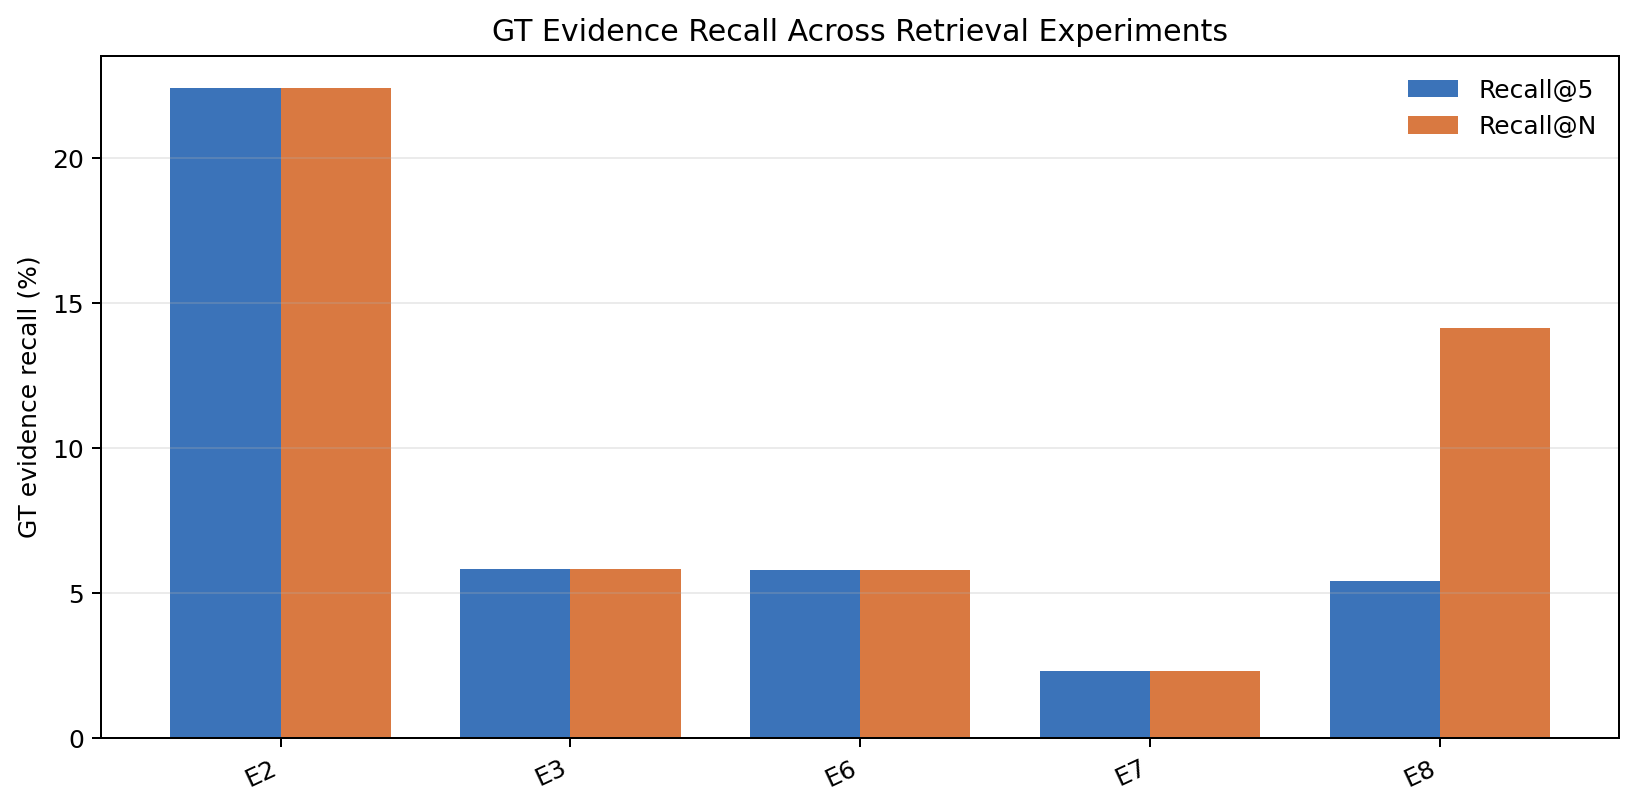
\includegraphics[width=0.82\linewidth]{e0_e13_recall.png}
\caption{GT 证据覆盖率对比。}
\label{fig:e0_e13_recall}
\end{figure}

\subsection{检索器对比实验}

为说明 Multi Query RAG(E8) 的提升来自查询构造和融合机制，而不是简单更换检索器，本文将 CLIP Retrieval(E3)、CLIP Rerank(E6) 和 MagicLens Retrieval(E7) 作为主要对比项。CLIP Retrieval(E3) 使用 CLIP 从完整 corpus 直接召回候选；CLIP Rerank(E6) 先由 CLIP 召回，再由 MagicLens 重排；MagicLens Retrieval(E7) 使用 MagicLens 直接从完整 corpus 召回候选。三者共同构成从“视觉近邻优先”到“关系指令优先”的能力谱系。

CLIP Retrieval(E3) 表明：仅使用 CLIP 从完整 corpus 中召回 Top-5 候选时，整体准确率为 50.41\%（682/1353），对应 Recall@5 为 5.85\%。分场景来看，CLIP Retrieval(E3) 在 \textit{Deformation}、\textit{Others} 和 \textit{Occlusion/Obstruction} 上相对稳定，但在 \textit{Temporal}、\textit{Scope} 和 \textit{Incomplete} 上明显偏弱。这说明 CLIP 能够较好保持视觉邻域，却不一定能找到对时间状态、范围判断或结构补全最有帮助的证据。

CLIP Rerank(E6) 对应“CLIP 粗召回 + MagicLens 重排”的混合方案，其整体准确率为 50.33\%，与 CLIP Retrieval(E3) 基本持平，Recall@5 为 5.80\%。这一结果不能简单解释为 MagicLens 失效，而说明当第一阶段候选覆盖主要由视觉近邻主导时，relation-aware reranking 的收益会受到候选集合本身的限制：如果 CLIP Top-5 中缺少真正 answer-useful evidence，重排器只能在有限候选内调整顺序。MagicLens Retrieval(E7) 评估 MagicLens 作为 direct retriever 的真实全库召回能力，其整体准确率为 47.97\%，Recall@5 仅为 2.31\%，略低于 CLIP Retrieval(E3)；但其在 \textit{Incomplete}、\textit{Biological} 与 \textit{Temporal} 等场景上的局部优势提示，MagicLens 的归纳偏好更接近结构补全、细粒度语义关系和时间关系，而非稳定保持实例级视觉邻域。

Multi Query RAG(E8) 在 MagicLens Retrieval(E7) 的基础上加入 Gemma~4 多维查询规划与 RRF 融合，整体准确率提升到 56.32\%，相对 MagicLens Retrieval(E7) 提升 8.35 个百分点，相对 CLIP Retrieval(E3) 提升 5.91 个百分点，相对 CLIP Rerank(E6) 提升 5.99 个百分点。Optimized Multi Query RAG(E11\_4) 进一步将整体准确率提升到 57.43\%，相对 Multi Query RAG(E8) 增加 15 道正确题，提升 1.11 个百分点。分场景上，Multi Query RAG(E8) 的最强信号来自 \textit{Others}，达到 80.00\%；Optimized Multi Query RAG(E11\_4) 在该场景进一步提升到 84.17\%，并在 \textit{Scope}、\textit{Temporal}、\textit{Incomplete} 与 \textit{Angle} 上均超过 Multi Query RAG(E8)。与此同时，Optimized Multi Query RAG(E11\_4) 在 \textit{Deformation}、\textit{Obstruction} 和 \textit{Biological} 上略有下降，说明减少一个查询维度会改变不同场景中的证据覆盖偏好。从召回角度看，Multi Query RAG(E8) 的最终 Recall@5 为 5.42\%，但融合前 Recall@N 达到 14.13\%，明显高于 MagicLens Retrieval(E7) 单路直检；这说明多维查询并不是简单“多检索几次”，而是在查询规划层面将主体、属性、背景、相似候选与局部细节拆成多条可融合证据链，从而缓解 MagicLens direct retrieval 的单路偏置。

为了进一步判断这种提升是否具有明确的场景指向，而不是由少数样本偶然拉高，下面继续比较各方法在九类任务中的表现。图~\ref{fig:corpus_scenario_compare} 采用柱状图逐类对照 CLIP Retrieval(E3)、CLIP Rerank(E6)、MagicLens Retrieval(E7)，便于观察不同单路方案的局部差异；图~\ref{fig:corpus_scenario_radar} 则把 Multi Query RAG(E8) 与 Optimized Multi Query RAG(E11\_4) 放回全部主要设置中，并在图例中相邻展示，帮助判断参数优化前后的场景能力变化。结合两图可以看出，多维查询的提升并不是在所有类别上平均展开的，而是更多体现在 \textit{Others}、\textit{Scope}、\textit{Temporal} 等更依赖查询拆解与证据互补的场景上。

\begin{figure}[!htb]
\centering
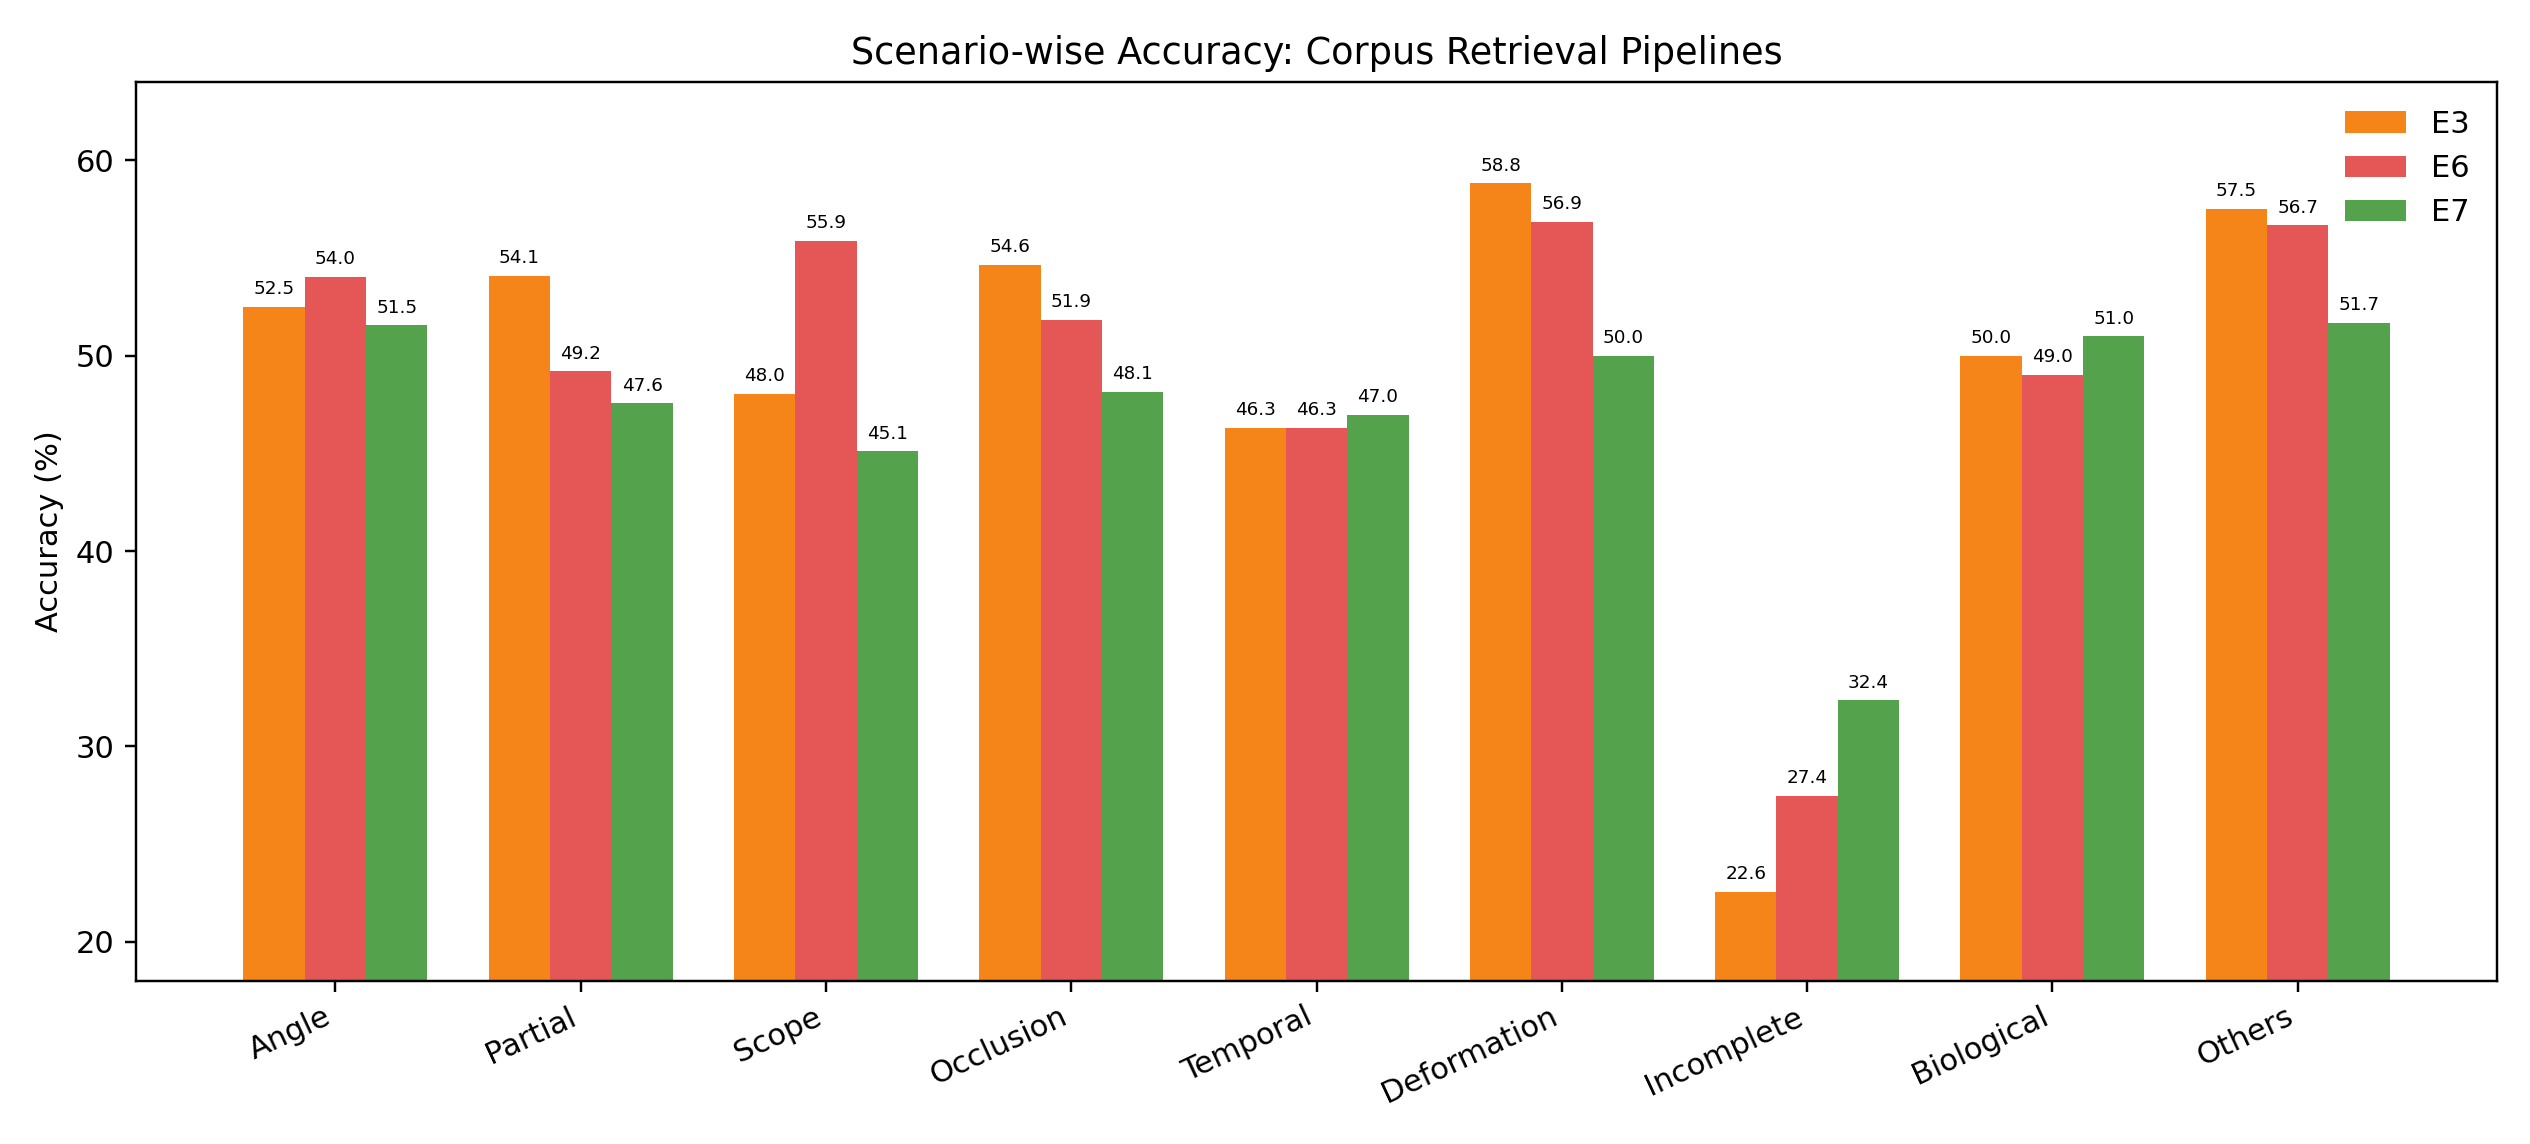
\includegraphics[width=\linewidth]{corpus_scenario_compare.png}
\caption{完整语料库检索基线分场景对比。}
\label{fig:corpus_scenario_compare}
\end{figure}

\begin{figure}[H]
\centering
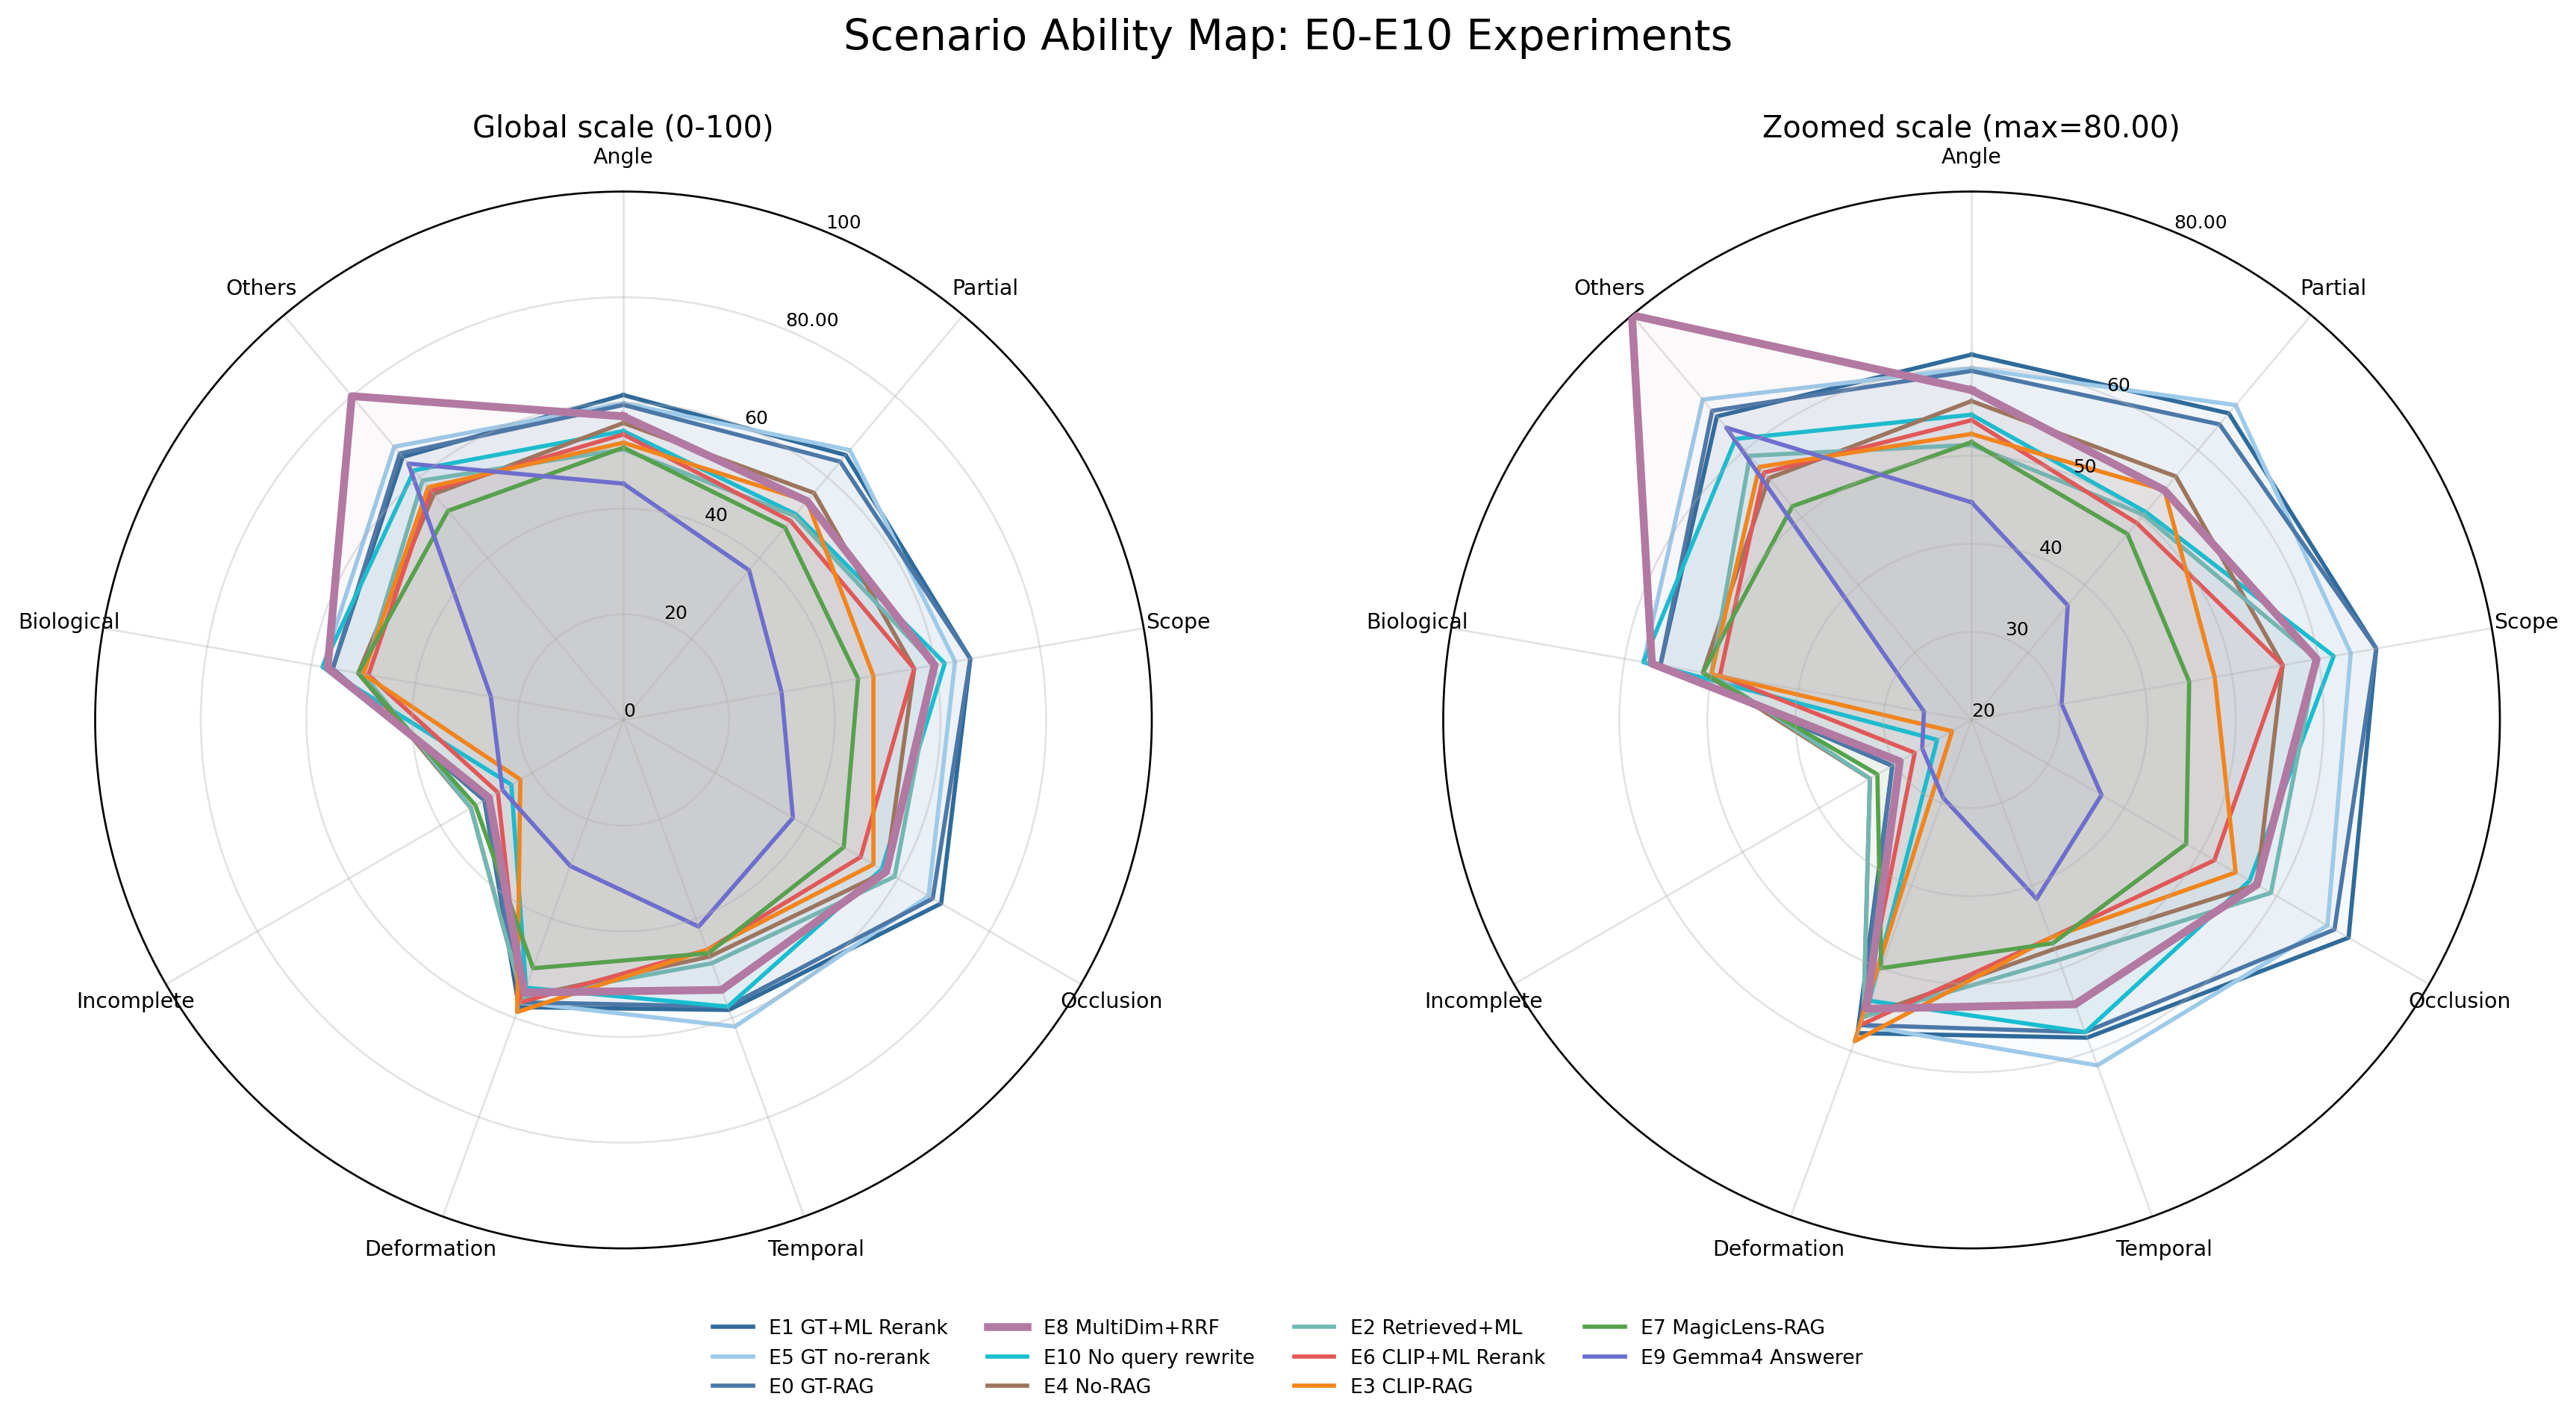
\includegraphics[width=0.88\linewidth]{e0_e10_radar.png}
\caption{主要方法分场景雷达对照。}
\label{fig:corpus_scenario_radar}
\end{figure}

总体来看，Corpus 线分析希望回答的核心问题是：“真实全库检索为什么难，以及 Multi Query RAG(E8) 为什么能比单路方法更好。”综合准确率、召回率和分场景结果，可以得到五点判断：第一，完整 corpus 检索下的粗召回误差不可忽略；第二，MagicLens 重排未能稳定改善 CLIP 的候选排序，主要受限于第一阶段候选覆盖；第三，MagicLens direct retrieval 并非整体优于 CLIP，但在少数关系性场景上具有可分析的局部优势；第四，Multi Query RAG(E8) 说明通过查询侧多维规划与列表融合，可以显著改善全库检索结果；第五，仅比较 overall accuracy 不足以解释检索器价值，必须结合候选结构、跨维重复命中与失败模式一并分析。

图~\ref{fig:error_share_by_scenario_compare} 进一步观察错误样本主要集中在哪些视觉困难类型，从而辅助判断方法改进是否只改变整体准确率，还是同时改变了失败样本的场景结构。

\begin{figure}[H]
\centering
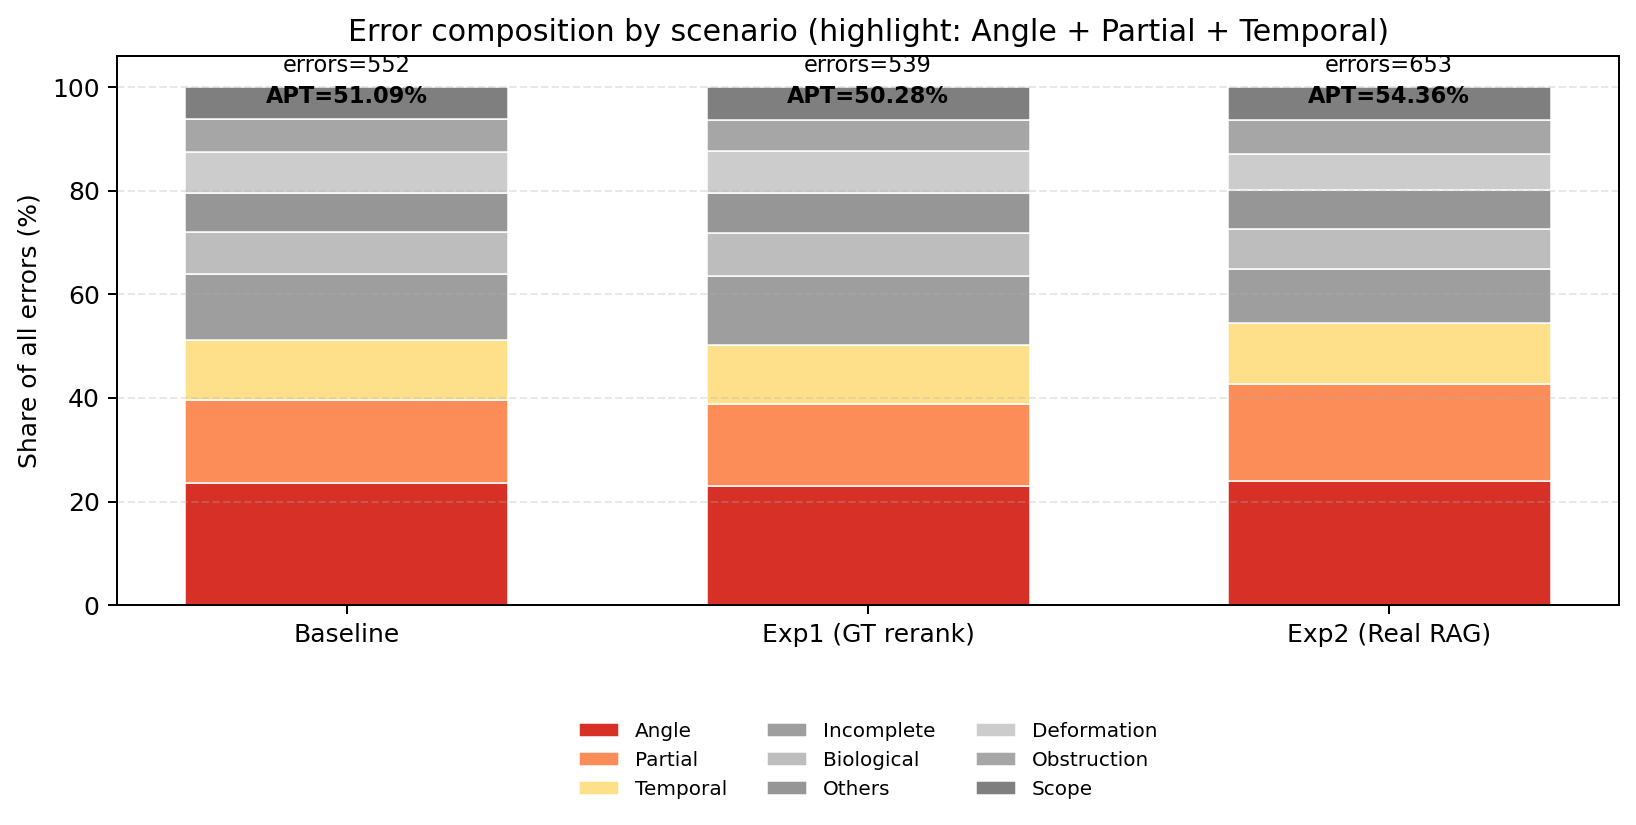
\includegraphics[width=0.88\linewidth]{error_share_by_scenario_compare.png}
\caption{场景错误占比分布。}
\label{fig:error_share_by_scenario_compare}
\end{figure}

\subsection{CLIP 与 MagicLens 检索差异}

前一节已经说明，CLIP Retrieval(E3) 与 MagicLens Retrieval(E7) 的整体准确率差距并不大，但这并不意味着两种检索器“找到了差不多的图”。恰恰相反，如果它们走向的是两套不同的候选分布，那么 Multi Query RAG(E8) 为什么需要把二者的优点重新组织起来，就必须回到检索集合本身去看。基于这一考虑，本节不再从最终答题结果出发，而是直接比较 CLIP 与 MagicLens 返回的候选集合结构。

对 1353 个样本逐一比较 Top-5 候选集合后可见，MagicLens 并非在 CLIP 的语义邻域内做轻微扰动，而是在大量 query 上走向了另一套检索偏好。

\subsubsection{检索集合差异}

这里首先要看的，不是谁的准确率略高，而是两种检索器究竟在多大程度上进入了同一个视觉证据邻域。只有先回答这个问题，后面才能解释 Multi Query RAG(E8) 为什么不能简单地被理解为“把某个更强的检索器直接换上去”。为此，图~\ref{fig:overview_plots} 从重合度、首位一致率和逐样本胜负三个角度给出全局概览，用来判断 CLIP 与 MagicLens 到底是在同一批候选上竞争，还是在走两条明显不同的检索路径。

在全部 1353 个样本中，CLIP 与 MagicLens 的 Top-5 候选平均仅重合 0.535 张；909 个样本（67.2\%）的 Top-5 候选完全没有重合，Top-5 完全一致的样本仅 1 个，Top-1 候选相同的样本也只有 204 个（15.1\%）。从答题正确率看，CLIP 正确 682 例，MagicLens 正确 649 例；逐样本胜负统计中，CLIP 胜出 152 例，MagicLens 胜出 119 例，两者都答对 530 例，都答错 552 例。上述结果说明，MagicLens 的确改变了检索证据分布，但这种改变并没有稳定转化为更高的问答准确率。

\begin{figure}[!htb]
\centering
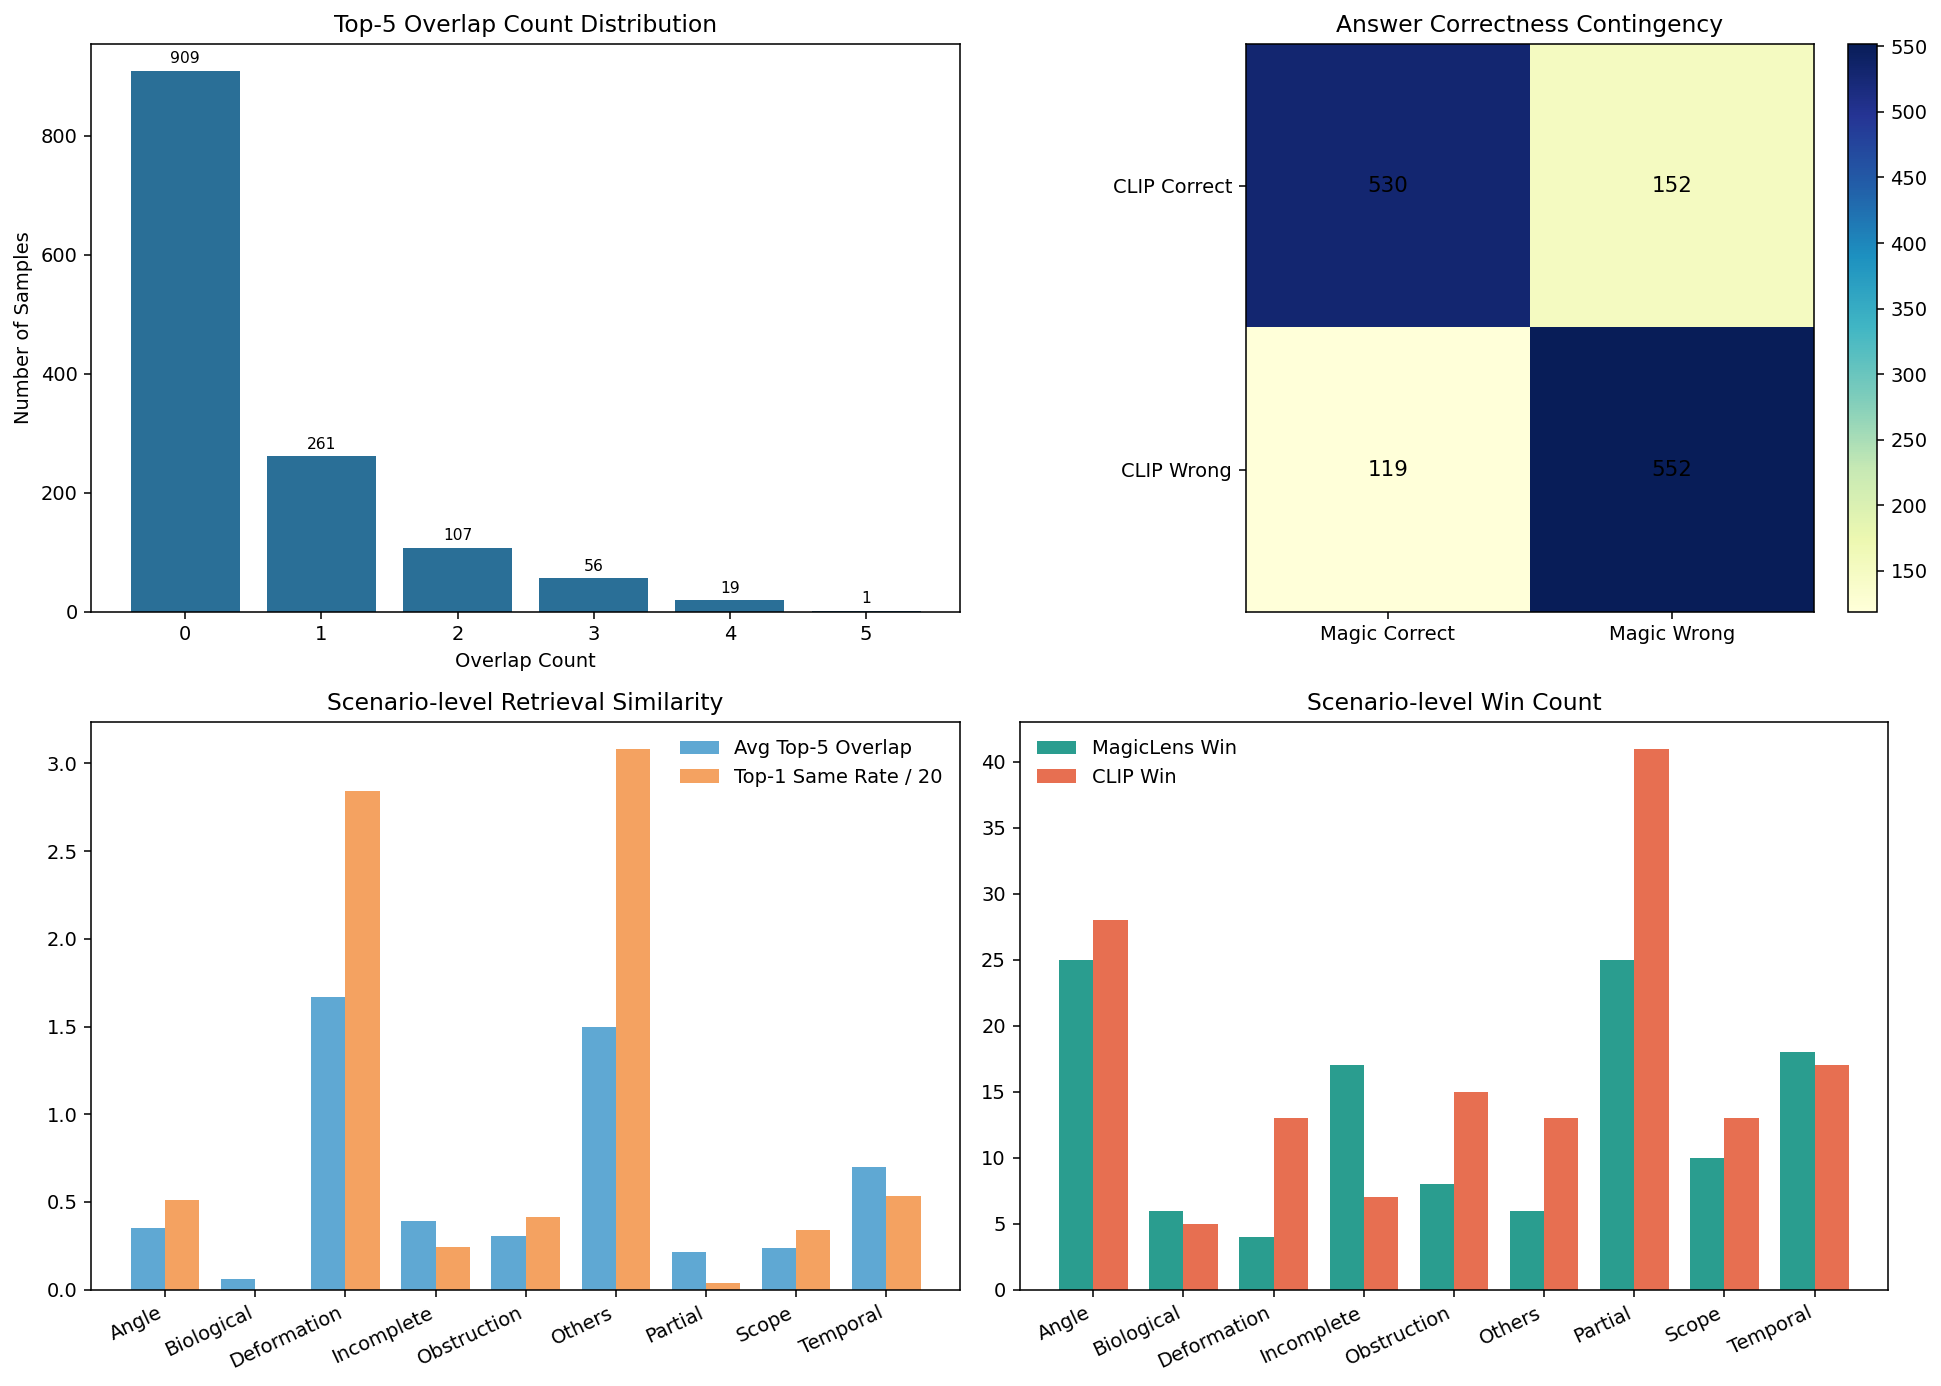
\includegraphics[width=\linewidth]{overview_plots.png}
\caption{CLIP 与 MagicLens 候选差异对比。}
\label{fig:overview_plots}
\end{figure}

\subsubsection{分场景检索差异}

仅有全局平均值还不够，因为不同场景对证据类型的要求本来就不一样。若要进一步理解 CLIP 和 MagicLens 的差异来自哪里，就需要把这种比较放回具体任务类型中，看它们在九类场景上的重合度和胜负关系是否存在稳定模式。基于这一目的，表~\ref{tab:scenario_retrieval_diff} 将检索集合差异拆解到各个场景中，用来回答“哪些场景更依赖视觉近邻，哪些场景更容易体现关系感知检索的优势”。

从 Top-5 重合度看，\textit{Deformation} 与 \textit{Others} 的重合度较高，说明这两类场景下 CLIP 与 MagicLens 的检索偏好更接近；而 \textit{Biological}、\textit{Partial} 与 \textit{Scope} 三类场景重合度极低，两者几乎检索出完全不同的候选集合。

\begin{table}[!htb]
\centering
\scriptsize
\caption{CLIP 与 MagicLens 在九类场景上的检索差异统计。}
\label{tab:scenario_retrieval_diff}
\begin{tabular}{lrrrrrr}
\toprule
\rowcolor{black!8}
\textbf{场景} & \textbf{$n$} & \textbf{Top-5 重合} & \textbf{Top-1 同(\%)} & \textbf{CLIP 准(\%)} & \textbf{ML 准(\%)} & \textbf{ML:CLIP 胜} \\
\midrule
Angle        & 322 & \cellcolor{red!10}0.354 & 10.25 & \cellcolor{blue!12}\textbf{52.48} & 51.55 & \cellcolor{blue!12}25:28 \\
Biological   & 102 & \cellcolor{red!20}\textbf{0.059} & \cellcolor{red!12}\textbf{0.00} & 50.00 & \cellcolor{green!15}\textbf{50.98} & \cellcolor{green!15}6:5  \\
Deformation  & 102 & \cellcolor{blue!15}\textbf{1.667} & \cellcolor{blue!18}56.86 & \cellcolor{blue!18}\textbf{58.82} & 50.00 & \cellcolor{blue!18}\textbf{4:13} \\
Incomplete   & 102 & \cellcolor{red!10}0.392 & 4.90 & 22.55 & \cellcolor{green!22}\textbf{32.35} & \cellcolor{green!22}\textbf{17:7} \\
Obstruction  & 108 & \cellcolor{red!10}0.306 & 8.33 & \cellcolor{blue!15}\textbf{54.63} & 48.15 & \cellcolor{blue!15}8:15 \\
Others       & 120 & \cellcolor{blue!12}1.500 & \cellcolor{blue!20}\textbf{61.67} & \cellcolor{blue!16}\textbf{57.50} & 51.67 & \cellcolor{blue!16}6:13 \\
Partial      & 246 & \cellcolor{red!15}0.215 & \cellcolor{red!10}0.81 & \cellcolor{blue!18}\textbf{54.07} & 47.56 & \cellcolor{blue!18}\textbf{25:41} \\
Scope        & 102 & \cellcolor{red!15}0.235 & 6.86 & \cellcolor{blue!10}\textbf{48.04} & 45.10 & \cellcolor{blue!10}10:13 \\
Temporal     & 149 & 0.698 & 10.74 & 46.31 & \cellcolor{green!12}\textbf{46.98} & \cellcolor{green!12}18:17 \\
\bottomrule
\end{tabular}
\vspace{0.25em}

\footnotesize
注：红色表示 CLIP 与 MagicLens 候选重合度很低，蓝色表示 CLIP 更优或二者候选更接近，绿色表示 MagicLens 更优；加粗为该列需要重点关注的极值或优势项。
\end{table}

从胜负计数看，MagicLens 的优势场景主要集中在 \textit{Incomplete} 和 \textit{Temporal}。其中，\textit{Incomplete} 场景要求系统判断缺失结构或补足不可见信息，更接近关系性与结构性推断，而非简单视觉相似匹配；\textit{Temporal} 场景则要求检索器捕捉状态变化和时间关系。相比之下，CLIP 在 \textit{Partial}、\textit{Deformation}、\textit{Obstruction} 与 \textit{Others} 上更稳定，说明这些场景更依赖局部视觉近邻或外观保持。该现象支持本文对二者能力边界的判断：CLIP 更适合作为覆盖稳定的粗召回器，MagicLens 更适合在关系性检索目标明确时发挥作用。

\subsubsection{Top-1 高频重复偏置}

在知道两种检索器会走向不同候选集合之后，还需要继续追问：MagicLens 的关系感知检索究竟是在扩大候选多样性，还是把大量查询集中吸附到少数高响应图像上。如果是后一种情况，那么它在某些场景中的局部优势就可能伴随着明显的候选集中偏置。为此，本节统计两种检索器 Top-1 候选的重复命中情况，并借助图~\ref{fig:top1_repeat_bias} 展示它们在头部集中度上的差异。

统计结果表明，MagicLens 存在明显的“原型图吸附”现象。CLIP 的 Top-1 候选分布较均匀，被重复命中 $\geq 5$ 次的图像仅 1 张；而 MagicLens 中有 57 张图像被 $\geq 5$ 个不同 query 命中为 Top-1，最高达到 39 次。图~\ref{fig:top1_repeat_bias} 将两种检索器的高频命中曲线放在同一坐标系下，并在右侧汇总最大重复次数、高频重复图像数、Top-10 集中度与唯一 Top-1 比例，从而更直接地展示 MagicLens 的头部集中现象。

\begin{figure}[!htb]
\centering

\includegraphics[width=\linewidth]{top1_repeat_bias.png}
\caption{Top-1 候选重复命中分布。}
\label{fig:top1_repeat_bias}
\end{figure}

这一现象说明，MagicLens 在当前 embedding 空间中存在少数高响应“原型图”，query 表征可能被开放式指令的语义维度过度牵引，从而削弱了 query image 的实例级约束。该问题会降低检索多样性，也限制下游模型获得差异化视觉证据的能力。

\subsection{时间代价与效率分析}

到这里为止，本文已经说明 Multi Query RAG(E8) 在效果上优于 CLIP Retrieval(E3)、CLIP Rerank(E6)、MagicLens Retrieval(E7)，但一个方法如果要具有现实意义，还需要回答另一个问题：这种收益是通过什么样的时间代价换来的，系统瓶颈究竟出现在检索侧还是生成侧。因此，本节转而考察 Multi Query RAG(E8) 的运行时间结构。

Multi Query RAG(E8) 全量过程记录显示，单样本平均总耗时为 42.58 秒，其中 Gemma~4 维度规划平均 17.59 秒，MagicLens 五路检索与 RRF 融合平均 3.40 秒，Gemma~4 对查询图和融合证据图生成描述平均 21.01 秒，LLaVA-OneVision 终答平均 0.34 秒。由此可见，Multi Query RAG(E8) 的性能收益主要来自查询侧规划和证据描述；真正的多路检索与融合阶段并不是瓶颈。

从部署角度看，若只保留“Gemma~4 多维规划 + MagicLens 分路召回 + RRF 融合 + LLaVA 终答”，而关闭证据描述步骤，平均耗时可显著下降。本文当前保留证据描述，是为了让日志和论文案例能够解释每张最终证据图对答题的潜在作用；在面向实际系统时，该模块可作为可解释性开关，而非必需的终答步骤。

\subsection{对比实验汇总}

表~\ref{tab:retriever_compare} 从检索器设置角度重新组织 CLIP Retrieval(E3)、CLIP Rerank(E6)、MagicLens Retrieval(E7)、Multi Query RAG(E8) 与 Optimized Multi Query RAG(E11\_4)。这里的重点不是重复列出主实验结果，而是把“仅替换检索器”和“同时改变查询构造与融合方式”这两类变化明确区分开。由此可以看出，单独更换检索器并不足以解决完整 corpus 检索问题，而 Multi Query RAG(E8)/Optimized Multi Query RAG(E11\_4) 的收益来自“查询构造 + 多路召回 + 融合”这一组合。

\begin{table}[!htb]
\centering
\scriptsize
\caption{MagicLens、CLIP 与多维查询侧扩展的对比结果。}
\label{tab:retriever_compare}
\resizebox{\textwidth}{!}{%
\begin{tabular}{lcccc}
\toprule
方法设置 & 整体准确率 & 分场景准确率 & 平均每样本时间 & 备注 \\
\midrule
CLIP Retrieval(E3) & 50.41 & Deformation 58.82 / Others 57.50 & 未统一统计 & 视觉语义粗召回 \\
CLIP Rerank(E6) & 50.33 & Deformation 56.86 / Others 56.67 & 未统一统计 & 混合检索，受 CLIP 候选覆盖限制 \\
MagicLens Retrieval(E7) & 47.97 & Incomplete 32.35 / Biological 50.98 & 未统一统计 & 指令关系检索，但存在单路偏置 \\
Multi Query RAG(E8) & 56.32 & Others 80.00 / Scope 59.80 & 42.58s & 初始五维查询配置 \\
Optimized Multi Query RAG(E11\_4) & 57.43 & Others 84.17 / Scope 62.75 & 29.97s & 参数优化后四维查询配置，当前最佳全量结果 \\
\bottomrule
\end{tabular}%
}
\end{table}

\section{消融实验}

\subsection{终答器消融：LLaVA 与 Gemma 4}

在明确了检索器与查询构造的作用之后，还需要进一步排除另一种可能：Multi Query RAG(E8) 的优势是否主要来自终答生成器本身，而非检索侧改进。为此，本小节固定 Multi Query RAG(E8) 的检索侧结构，仅替换最终答题器，专门观察同一组检索证据在不同 VLM 下的利用差异。

为尽量将性能变化归因于检索器与查询构造环节，本文前述 GT RAG(E0) 至 Multi Query RAG(E8) 主实验统一采用 LLaVA-OneVision 作为终答生成器，而将 Gemma~4 主要用于维度规划、查询重写与证据描述。这一设置的优点是变量控制清楚，能够避免“检索器变化”与“生成器变化”同时发生，从而使主实验更容易解释。与此同时，本文在系统实现层面已经为 Gemma~4 直接承担终答生成任务预留接口，因此 Gemma Answerer(E9) 将 Multi Query RAG(E8) 的最终答题器由 LLaVA-OneVision 替换为 Gemma~4~E2B-it，用于观察同一类检索证据在不同 VLM 终答器下的利用差异。

Gemma Answerer(E9) 保持 Multi Query RAG(E8) 的检索侧主架构不变：Gemma~4 仍负责生成五条多维检索 query，MagicLens 仍对每一维执行 full corpus Top-5 检索，RRF 仍融合得到最终 Top-5 证据，Gemma~4 仍生成查询图与证据图的辅助描述；唯一主要变量是最终多选题答题器。全量 1353 个样本上，Gemma Answerer(E9) 的 overall accuracy 为 38.95\%（527/1353），明显低于 Multi Query RAG(E8) 的 56.32\%（762/1353），下降 17.37 个百分点。Gemma Answerer(E9) 的最终答题阶段没有运行异常，选项抽取失败仅 4 题（0.30\%），因此性能下降不能主要归因于格式错误，而应归因于 Gemma~4~E2B-it 在当前多图证据组织方式下的判别与证据整合能力不足。

分场景看，Gemma Answerer(E9) 仍在 \textit{Others} 上取得最高值 63.33\%，但相比 Multi Query RAG(E8) 的 80.00\% 下降 16.67 个百分点；\textit{Angle} 与 \textit{Temporal} 分别为 44.72\% 和 41.61\%，是相对较稳的两类；下降最明显的是 \textit{Biological}、\textit{Scope} 与 \textit{Deformation}，分别只有 25.49\%、30.39\% 和 29.41\%。逐样本对照进一步显示，Multi Query RAG(E8) 与 Gemma Answerer(E9) 同时答对 376 题，Multi Query RAG(E8) 对而 Gemma Answerer(E9) 错 386 题，Multi Query RAG(E8) 错而 Gemma Answerer(E9) 对 151 题，两者同时答错 440 题。这说明 Gemma~4 并非完全不能利用检索证据，但其收益不足以抵消大量 Multi Query RAG(E8) 正确样本上的退化。

\begin{table}[!htb]
\centering
\scriptsize
\caption{LLaVA 与 Gemma~4 终答生成器对比结果。}
\label{tab:generator_compare}
\resizebox{\textwidth}{!}{%
\begin{tabular}{lcccc}
\toprule
终答生成器 & 检索设置 & 整体准确率 & 平均终答耗时 & 终答失败率 \\
\midrule
LLaVA-OneVision & Multi Query RAG(E8)：Gemma~4 多维查询 + MagicLens + RRF & 56.32 & 0.34s & 0.00\% \\
Gemma~4~E2B-it & Gemma Answerer(E9)：同 Multi Query RAG(E8) 检索侧，仅替换终答器 & 38.95 & 1.46s & 0.30\%（选项抽取失败） \\
\bottomrule
\end{tabular}%
}
\end{table}

\subsection{查询重写消融}

Multi Query RAG(E8) 的另一个关键因素是查询重写。本文在查询链中引入查询重写模块，目的不是把原始问题改写得更自然，而是把其从“更接近生成任务的语言形式”转换为“更接近图像检索需求的中间表示”。Raw Query(E10) 直接把原始 question 与 choices 作为单条 MagicLens 检索指令，Multi Query RAG(E8) 则由 Gemma~4 生成五条互补检索维度并进行 RRF 融合。二者保持检索器、候选库和下游生成器不变，主要差异在查询构造方式。

结果显示，Raw Query(E10) 的整体准确率为 53.51\%，低于 Multi Query RAG(E8) 的 56.32\%。从召回角度看，Raw Query(E10) 的 Recall@5 与 Recall@N 均为 5.00\%；Multi Query RAG(E8) 虽然最终 Recall@5 只有 5.42\%，但融合前 Recall@N 达到 14.13\%。这说明多维查询重写的主要贡献不是让最终 Top-5 直接覆盖更多 GT，而是显著扩大融合前候选池中的有效证据覆盖，为后续融合和终答提供更大的证据空间。

\begin{table}[!htb]
\centering
\scriptsize
\caption{查询重写模块消融结果。Raw Query(E10) 直接使用原始问题与选项作为单条检索指令，Multi Query RAG(E8) 使用 Gemma~4 生成五条互补查询并进行 RRF 融合。}
\label{tab:ablation_rewrite}
\resizebox{\textwidth}{!}{%
\begin{tabular}{lccccc}
\toprule
设置 & 整体准确率 & R@5 & R@N & 平均检索耗时 & 备注 \\
\midrule
Raw Query(E10) & 53.51 & 5.00 & 5.00 & 0.71s & 原始问题直接检索 \\
Multi Query RAG(E8) & 56.32 & 5.42 & 14.13 & 3.40s & Gemma~4 五维查询 + RRF \\
\bottomrule
\end{tabular}%
}
\end{table}

\section{参数实验}

\subsection{多维查询参数概述}

本文初始全量运行采用 $N=5$ 个查询维度、每维 Top-$K_{\mathrm{dim}}=5$、最终 Top-$K_{\mathrm{final}}=5$ 的设置，并使用 RRF 进行多列表融合。该设置对应 Multi Query RAG(E8) baseline。参数实验的目的不是穷举所有组合，而是观察查询维度数和每维候选数如何影响候选结构、准确率与运行成本，并在此基础上验证是否存在比 Multi Query RAG(E8) 更合适的全量配置。

Multi Query RAG(E8) 的提升不仅来自“多检索几次”，还来自“怎样把多路检索结果组织成一个最终候选集合”。因此，本小节进一步关注融合阶段本身：RRF 到底改变了什么样的候选结构，它是单纯扩大了候选池，还是让不同维度对同一关键证据形成了更稳定的支持。

在 Multi Query RAG(E8) 中，查询侧扩展并不是到多路召回为止，后续如何把这些结果组织成最终证据集合，同样决定了系统最后看到的视觉条件。本文当前全量结果采用 RRF 作为默认融合策略。统计结果显示，Multi Query RAG(E8) 的整体准确率为 56.32\%，融合前候选池平均包含 25 个输入候选、约 19.35 个唯一候选，唯一候选比例为 77.40\%；同时 94.75\% 的样本存在跨维重复命中。这说明 RRF 的作用并不是简单扩大候选数量，而是在保留一定多样性的同时，使多个维度能够对同一候选形成共识，从而重塑最终的候选结构。

数值统计能够告诉我们“结果如何”，但很难直接说明“系统究竟看到了什么图、这些图之间是什么关系”。因此，在讨论候选结构之后，还需要通过可视化结果把检索阶段的中间状态直观呈现出来，使前面的统计判断能够回到具体样本上得到验证。Multi Query RAG(E8) 可以输出各维度 Top-1 横向拼贴、分维 Top-$K$ 网格总览、查询图与融合后 Top-5 证据拼图等可视化结果。这些图像用于观察不同维度间是否重复命中相同候选、判断融合前后证据多样性是否提升，以及对照错误案例分析模型实际接收到的视觉条件。

本小节展示 Multi Query RAG(E8) 已生成的代表性过程图。对于正确样本，重点展示多维查询是否确实召回了互补证据；对于错误样本，重点展示失败是源于候选图像偏离任务需求、候选之间高度冗余，还是下游模型未能利用已有证据；对于边界样本，则重点展示“检索阶段已经逼近正确视觉邻域，但最终选择仍然失败”的情况，以区分检索瓶颈与生成瓶颈。与“维度 $\times$ Top-$K$”网格相关的可视化已在第~\ref{sec:e8_example_qs0}~节的图~\ref{fig:e8_qs0_viz}(b) 中给出，因此本节不再重复展示同一图像。结合该图可以看到，不同维度之间既存在对同一候选的重复命中，也保留了部分互补候选，这正是后续 RRF 融合能够形成跨维共识而非简单拼接列表的基础。

\subsection{分层采样参数扫描}

由于 Multi Query RAG(E8) 全量运行成本较高，本文没有在 1353 个测试样本上穷举所有参数组合，而是在九个场景中各采样 10 个样本，构成 90 条分层样本，对查询维度数 $N$ 和每维召回数 $K_{\mathrm{dim}}$ 进行局部扫描。所有参数实验使用同一批 90 个样本、同一图像语料库、同一 MagicLens 检索器、同一 RRF 融合策略和同一 LLaVA-OneVision 终答器，因此 P01--P08 之间可以进行逐样本成对比较。需要说明的是，Multi Query RAG(E8) baseline 是 1353 条全量结果，只作为主实验参考；本小节中的 P01--P08 更适合解释参数趋势，而不用于替代全量主结果。

\begin{table}[!htbp]
\centering
\fontsize{7.8pt}{8.6pt}\selectfont
\setlength{\tabcolsep}{4pt}
\renewcommand{\arraystretch}{0.86}
\caption{多维查询参数扫描结果。}
\label{tab:param_sweep_results}
\resizebox{\textwidth}{!}{%
\begin{tabular}{lcccccc}
\toprule
实验 & $N$ & $K_{\mathrm{dim}}$ & 准确率 & 正确数 & 平均总耗时 & 平均唯一候选数 \\
\midrule
P01 & 1 & 5 & 56.67 & 51/90 & 21.21s & 5.00 \\
P02 & 2 & 5 & 58.89 & 53/90 & 21.38s & 8.94 \\
P03 & 3 & 5 & 53.33 & 48/90 & 24.41s & 12.51 \\
P04 & 4 & 5 & 58.89 & 53/90 & 27.53s & 15.41 \\
\midrule
P05 & 5 & 1 & 58.89 & 53/90 & 29.00s & 4.03 \\
P06 & 5 & 2 & 55.56 & 50/90 & 32.54s & 7.63 \\
P07 & 5 & 3 & 55.56 & 50/90 & 33.43s & 11.41 \\
P08 & 5 & 4 & \best{61.11} & \best{55/90} & 32.73s & 15.07 \\
\bottomrule
\end{tabular}%
}
\end{table}

表~\ref{tab:param_sweep_results} 显示，查询维度数和每维召回数都不是越大越好。在维度数扫描中，$N=2$ 与 $N=4$ 都达到 58.89\%，但 $N=2$ 的平均总耗时仅为 21.38 秒，明显低于 $N=4$ 的 27.53 秒，因此从成本收益看 $N=2$ 是更经济的设置。$N=3$ 反而下降到 53.33\%，说明额外维度可能引入噪声候选，或者不同维度之间并未形成有效互补。该结果提醒我们，多维查询的关键不只是增加检索次数，而是让各维度真正覆盖互补的证据需求。

在每维召回数扫描中，$K_{\mathrm{dim}}=4$ 的 P08 达到 61.11\%，是本轮参数实验中最高的设置。相比 $K_{\mathrm{dim}}=2$ 与 $K_{\mathrm{dim}}=3$，P08 的平均唯一候选数增加到 15.07，并且准确率同时提高，说明每维保留 4 个候选时，融合阶段获得了更充分的互补证据。相比之下，$K_{\mathrm{dim}}=2/3$ 只增加了候选数量，却未稳定转化为更高准确率，表明中等规模候选池可能先暴露噪声，再在更大候选覆盖下获得收益。

为了进一步确认参数变化带来的收益是否来自同一批样本上的真实改进，本文统计了关键设置之间的逐题成对差异。P08 相比 P05 新增 4 题正确、损失 2 题正确，净增 2 题；相比 P06 和 P07 均新增 5 题正确且没有损失已有正确题，净增 5 题。因此，P08 的优势并不只是总体比例波动，而是能在同一批样本上覆盖更多此前失败的题目。维度数扫描中，P02 相比 P01 新增 7 题正确、损失 5 题正确，净增 2 题；P04 相比 P03 新增 8 题正确、损失 3 题正确，说明不同维度数的收益具有明显样本选择性。

分场景结果进一步表明，不同任务类型对参数的敏感性并不一致。Angle 和 Scope 在多数设置下仍较低，说明这两类问题可能更依赖查询表达质量或证据选择机制，而不是单纯增加候选数量；Biological 与 Others 在 P05/P08 上表现较好，说明更多候选或更合适的每维召回数能够改善细粒度类别相关问题；Incomplete 在 P02 上达到 70.00\%，但 P08 只有 50.00\%，说明缺失结构类问题未必适合无条件扩大候选池。总体来看，参数扫描支持两点判断：第一，P08（$N=5,K_{\mathrm{dim}}=4$）是本轮准确率最高的默认配置候选；第二，若需要控制推理成本，P02（$N=2,K_{\mathrm{dim}}=5$）提供了更好的速度与准确率折中。

\begin{table}[!htbp]
\centering
\fontsize{7.8pt}{8.6pt}\selectfont
\setlength{\tabcolsep}{4pt}
\renewcommand{\arraystretch}{0.86}
\caption{参数扫描运行时间结构。}
\label{tab:param_sweep_time}
\resizebox{\textwidth}{!}{%
\begin{tabular}{lccccc}
\toprule
实验 & 平均总耗时 & 维度生成 & 检索融合 & 证据描述 & 终答生成 \\
\midrule
P01 & 21.21s & 5.53s & 0.75s & 14.64s & 0.22s \\
P02 & 21.38s & 5.47s & 1.40s & 14.24s & 0.21s \\
P03 & 24.41s & 7.77s & 2.02s & 14.33s & 0.23s \\
P04 & 27.53s & 10.17s & 2.66s & 14.39s & 0.23s \\
P05 & 29.00s & 12.48s & 3.29s & 12.83s & 0.34s \\
P06 & 32.54s & 12.73s & 3.29s & 16.04s & 0.41s \\
P07 & 33.43s & 13.02s & 3.35s & 16.59s & 0.41s \\
P08 & 32.73s & 12.78s & 3.29s & 16.18s & 0.41s \\
\bottomrule
\end{tabular}%
}
\end{table}

表~\ref{tab:param_sweep_time} 说明，系统主要耗时来自 Gemma~4 的维度生成和证据描述，MagicLens 检索与 RRF 融合本身并不是主要瓶颈。随着 $N$ 增加，维度生成与检索融合耗时上升较明显；随着 $K_{\mathrm{dim}}$ 增加，耗时变化更多体现在最终候选描述阶段。结合准确率结果，本文后续默认仍保留多维融合路线，但需要继续通过全量实验验证抽样阶段的参数趋势。

\subsection{Optimized Multi Query RAG 全量验证}

分层采样实验中，P08 在 90 条样本上取得最高准确率，但 P04（$N=4,K_{\mathrm{dim}}=5$）在维度数扫描中与 P02/P05 同分，且平均唯一候选数为 15.41，接近 Multi Query RAG(E8) 全量运行中的候选结构。为了验证减少一个查询维度是否能够降低噪声并改善全量性能，本文进一步运行 Optimized Multi Query RAG(E11\_4) 全量实验。该实验保持 MagicLens 检索器、RRF 融合、最终 Top-5、证据描述模块和 LLaVA-OneVision 终答器不变，仅将查询维度数从 5 改为 4。

\begin{table}[H]
\centering
\scriptsize
\caption{Multi Query RAG(E8) 与 Optimized Multi Query RAG(E11\_4) 的全量参数验证结果。}
\label{tab:e11_4_full_compare}
\resizebox{\textwidth}{!}{%
\begin{tabular}{lccccccc}
\toprule
实验 & $N$ & $K_{\mathrm{dim}}$ & 正确数 & 准确率 & 平均总耗时 & 维度生成 & 检索融合 \\
\midrule
Multi Query RAG(E8) & 5 & 5 & 762/1353 & 56.32 & 42.58s & 17.59s & 3.40s \\
Optimized Multi Query RAG(E11\_4) & 4 & 5 & \best{777/1353} & \best{57.43} & \best{29.97s} & \best{10.67s} & \best{2.70s} \\
\bottomrule
\end{tabular}%
}
\end{table}

表~\ref{tab:e11_4_full_compare} 显示，Optimized Multi Query RAG(E11\_4) 在全量 1353 个样本上达到 57.43\%，比 Multi Query RAG(E8) 的 56.32\% 提升 1.11 个百分点，对应多答对 15 题。同时，Optimized Multi Query RAG(E11\_4) 的平均总耗时为 29.97 秒，低于 Multi Query RAG(E8) 的 42.58 秒；其中维度生成耗时从 17.59 秒降至 10.67 秒，检索融合耗时从 3.40 秒降至 2.70 秒。该结果说明，多维查询并非维度越多越好。额外的第五个维度虽然扩大了融合前候选池，但也可能引入噪声候选并增加描述成本；四维查询在证据覆盖与噪声控制之间取得了更好的折中。

从分场景看，Optimized Multi Query RAG(E11\_4) 相比 Multi Query RAG(E8) 在 \textit{Others}、\textit{Scope}、\textit{Temporal}、\textit{Incomplete} 与 \textit{Angle} 上分别提升 4.17、2.95、2.69、1.96 和 1.87 个百分点；但在 \textit{Deformation}、\textit{Obstruction} 与 \textit{Biological} 上分别下降 3.92、1.85 和 0.98 个百分点。这表明四维配置并不是在所有场景中统一占优，而是通过减少噪声维度提升了多数场景的整体稳定性。综合准确率与耗时，本文将 Optimized Multi Query RAG(E11\_4) 作为参数优化后的最终配置，Multi Query RAG(E8) 则作为初始五维配置和消融参照保留。

\subsection{单维与多维查询对比}

在确认查询重写本身有效之后，还需要进一步回答另一个更细的问题：Multi Query RAG(E8) 的提升究竟来自“改写得更好”，还是来自“维度数量变多、证据来源变得互补”。因此，本小节继续比较单维查询与多维查询两种设置，重点观察多维结构本身是否带来了候选覆盖上的实质变化。

\begin{table}[!htbp]
\centering
\fontsize{7.8pt}{8.6pt}\selectfont
\setlength{\tabcolsep}{4pt}
\renewcommand{\arraystretch}{0.86}
\caption{单维查询与多维查询比较结果。}
\label{tab:ablation_multidim}
\resizebox{\textwidth}{!}{%
\begin{tabular}{lccccc}
\toprule
设置 & 整体准确率 & R@5 & R@N & 候选结构 & 备注 \\
\midrule
Raw Query(E10) & 53.51 & 5.00 & 5.00 & 单路 Top-5 & 原始问题直接检索 \\
Multi Query RAG(E8) & 56.32 & 5.42 & 14.13 & 25 输入 / 19.35 唯一 & 五维查询 + RRF \\
\bottomrule
\end{tabular}%
}
\end{table}

表~\ref{tab:ablation_multidim} 显示，Multi Query RAG(E8) 相比 Raw Query(E10) 的整体准确率从 53.51\% 提升到 56.32\%，融合前 Recall@N 从 5.00\% 提升到 14.13\%。这说明五维查询与 RRF 的主要作用是扩大融合前候选覆盖，而不是单纯改写原问题。其候选池平均包含 25 个输入候选、约 19.35 个唯一候选，且 94.75\% 的样本存在跨维重复命中。

\chapter{总结}

本文围绕 vision-centric mRAG 中“系统究竟应当检索什么样的视觉证据”这一核心问题展开研究。与将检索简单理解为寻找视觉上最相似图像的思路不同，本文强调，多模态问答中的关键不只是找到“像”的图像，而是找到能够真正支撑回答的问题相关证据。基于这一判断，本文从问题导向证据检索的角度重新审视 MRAG-Bench，指出 benchmark 自带候选与人工标注证据之间存在明显覆盖缺口，从而说明 vision-centric mRAG 的瓶颈并不只是后续生成模型如何作答，更在于检索阶段能否把正确证据带到模型面前。

在此基础上，本文创新性地提出了面向问题导向证据召回的混合检索思路：以 CLIP 提供稳定的视觉邻域召回，以 MagicLens 补充关系感知能力，并进一步通过多维查询生成与结果融合增强复杂问题下的证据搜索能力。实验结果表明，单纯依赖局部重排或单一路径检索都难以稳定解决 vision-centric mRAG 中的证据缺失问题，而将候选覆盖、关系建模与查询表达协同起来，能够更有效地提升非 GT 条件下的检索表现。进一步的参数实验表明，多维查询并非维度越多越好；四维查询配置 Optimized Multi Query RAG(E11\_4) 在全量验证中达到 57.43\%，高于五维 Multi Query RAG(E8) 的 56.32\%，同时平均耗时更低，说明查询维度需要在证据覆盖和噪声控制之间折中。更重要的是，本文不仅比较了不同方法“谁更好”，还进一步揭示了它们“为什么会成功或失败”，从而把研究重点从结果优劣推进到机制理解。

从更广泛的意义上看，vision-centric mRAG 的价值并不只在于提高若干基准上的问答准确率，更在于推动多模态系统从“依赖参数记忆作答”走向“依赖外部证据作答”。本文的工作表明，只有当检索目标真正从“相似图像”转向“有效证据”时，多模态检索增强生成系统才可能获得更强的可解释性、可验证性与实际应用价值。

\bibliographystyle{gbt7714-numerical}
\bibliography{../doc/开题报告LaTeX/ref_ordered}

\chapter*{致\quad 谢}
\addcontentsline{toc}{chapter}{致\texorpdfstring{\quad}{ }谢}
本文从选题、实验设计、代码实现到论文整理，得到了导师宋歌老师的耐心指导和持续帮助。在研究推进过程中，老师不仅在研究方向和论文结构上给予了明确建议，也在实验组织、问题拆分和结果分析方面提供了很多启发，使我能够逐步把零散的实验记录整理为较完整的研究主线。在此谨向宋老师表示诚挚的感谢。

同时，感谢实验室和项目协作过程中给予帮助的同学与朋友。大家在数据处理、模型运行、图表讨论和论文修改中的交流，使我在面对复杂问题时能够不断修正思路、保持推进。也感谢学院在本科阶段提供的课程训练与科研实践机会，使我能够逐步完成从课程学习到研究实践的过渡。

最后，感谢家人在本科阶段给予的理解、支持与鼓励。正是因为这些帮助，我才能够持续投入到本课题的学习、实验与写作之中，并完成本文工作。


\cleardoublepage
\chapter*{本科期间主要研究成果}

\section*{发表论文}
\begin{enumerate}[leftmargin=2em]
\item \textcolor{red!75!black}{\textbf{Ziyan Shi}}, Y Gu, H Cui, et al. From Machine Learning to Multimodal Models: The AI Revolution in Enzyme Engineering. \textit{BioDesign Research}, 2025. DOI: \href{https://doi.org/10.1016/j.bidere.2025.100044}{10.1016/j.bidere.2025.100044}. （SCI，影响因子 4.7，JCR Q1）
\item Yuan S, Peng N, \textcolor{red!75!black}{\textbf{Shi Z}}, et al. Detection of algal tiny objects based on morphological features. \textit{Concurrency and Computation: Practice and Experience}, 2024:e8128. DOI: \href{https://onlinelibrary.wiley.com/doi/10.1002/cpe.8128}{10.1002/cpe.8128}. （SCI/SCIE，中科院 4 区，JCR Q2）
\item S. Yuan, N. Peng, Z. \textcolor{red!75!black}{\textbf{Shi}}, Y. Gu and B. Sun. ``MAgic: A Morphable Attention Based Algal Tiny Object Detection Model,'' in \textit{2023 10th International Conference on Behavioural and Social Computing (BESC)}, Larnaca, Cyprus, 2023, pp.~1--8. DOI: \href{https://ieeexplore.ieee.org/document/10386562}{10.1109/BESC59560.2023.10386562}. （EI，IEEE）
\end{enumerate}

\section*{完成项目}
\begin{enumerate}[leftmargin=2em]
\item 参与基于 YOLOv8 的藻类微小目标检测研究，围绕形态学特征建模、注意力机制设计与数据集构建开展实验，形成 conference 与 journal 两条成果线。
\item 参与酶工程方向的 AI for Science 研究，围绕酶功能预测、酶工程任务建模与多模态模型在生命科学中的应用开展文献调研与综述写作，形成 \textit{BioDesign Research} 论文成果。
\item 参与酶学编号预测（EC number prediction）相关项目，面向分子表示、反应式建模与酶功能分类问题进行数据处理、模型实验与结果分析。
\item 参与实验室自动化方向项目，基于 Opentrons 平台完成实验流程编排与自动化脚本编写，支持 PCR 等湿实验步骤的标准化执行。
\item 参与脑启发计算方向项目，围绕 BrainPy 建模、神经形态计算平台使用与相关学术交流活动开展学习与实践。
\item 参与基于 THz 的脑机接口（BCI）方向项目，围绕多模态信号整合、设备方案设计与算法分析开展前期研究与实验探索。
\item 参与 iGEM Competition 与 iGEM Hackathon 相关项目，完成队伍协作、方案设计与竞赛实践。
\end{enumerate}

\end{document}
